%%%%%% IMPORTAÇÃO DOS PACOTES %%%%%%
\documentclass[
	% -- opções da classe memoir --
	12pt,				% tamanho da fonte
	openright,			% capítulos começam em páginas ímpar (insere página vazia caso preciso)
	oneside,			% para impressão em verso e anverso. Oposto a oneside
	a4paper,		% tamanho do papel.
	% -- opções da classe abntex2 --
	% chapter=TITLE,		% títulos de capítulos convertidos em letras maiúsculas
	% section=TITLE,		% títulos de seções convertidos em letras maiúsculas
	%subsection=TITLE,	% títulos de subseções convertidos em letras maiúsculas
	%subsubsection=TITLE,% títulos de subsubseções convertidos em letras maiúsculas
	% -- opções do pacote babel --
    brazil,				% o último idioma é o principal do documento
	english,			% idioma adicional para hifenização
	%french,			% idioma adicional para hifenização
	%spanish,			% idioma adicional para hifenização
	sumario=tradicional,
	]{abntex2}

% --------------- PACOTES -----------------%
%%%%% conflict with float package, loaded by one of the packages bellow.
% \usepackage{floatrow} % pacote para criar ambientes float genéricos
% \floatsetup[table]{style=plaintop} % poe legendas de tabelas em cima.

% Pacotes fundamentais
\usepackage{cmap}				% Mapear caracteres especiais no PDF
\usepackage{lmodern}			% Usa a fonte Latin Modern
% \usepackage{fontspec}
% \setmainfont{Computer Modern Roman}

\usepackage[T1]{fontenc}		% Selecão de códigos de fonte. hifenação correta.
\usepackage[utf8]{inputenc}		% Codificacao do documento (conversão automática dos acentos)
\usepackage{lastpage}			% Usado pela Ficha catalográfica
\usepackage{indentfirst}		% Indenta o primeiro parágrafo de cada seção.
\usepackage{xcolor}				% Controle das cores
\usepackage[pdftex]{graphicx}	% Inclusão de gráficos
\graphicspath{{figures/}}
\usepackage{subcaption}
\usepackage{epstopdf}           % Pacote que converte as figuras em eps para pdf


% Pacotes adicionais, usados apenas no âmbito do Modelo Canônico do abnteX2
\usepackage{nomencl}
\usepackage{amssymb}   % more symbols
\usepackage{amsmath}   % usado para ter o environment pmatrix, align
\usepackage{mathtools} % usado para ter o environment pmatrix*
\usepackage{mathrsfs}  % usado para ter o curly H
\usepackage{xfrac}     % usado para ter o comando \sfrac
\usepackage{bbm}
% \usepackage[chapter]{algorithm}
% \usepackage{algorithmic}
\usepackage{multirow}
\usepackage{dcolumn}        % para ter colunas alinhadas no ponto
\usepackage{rotating}       % to make sideways figures and tables
\usepackage{pdfpages}       % insere páginas pdf no arquivo
\usepackage{siunitx}        % pacote para padronizar display de números e unidades

\usepackage[brazilian,hyperpageref]{backref}	 % Paginas com as citacões na bibl

\usepackage[toc,acronym,nomain,nogroupskip,nonumberlist]{glossaries}%nonumberlist
\newacronym{linac}{LINAC}{Linear Accelerator}
\newacronym{cnpem}{CNPEM}{National Center for Research in Energy and Materials}
\newacronym{lnls}{LNLS}{Brazilian Synchrotron Light Laboratory}
\newacronym{3gls}{3$^\text{rd}$ GLS}{Third Generation Light Sources}
\newacronym{4gls}{4$^\text{th}$ GLS}{Fourth Generation Light Sources}
\newacronym{bsc}{BSC}{Beam Stay Clear}
\newacronym{supcond}{SC-RF}{Superconducting RF Cavity}
\newacronym{lhs}{l.h.s.}{left hand side}
\newacronym{rhs}{r.h.s.}{right hand side}
\newacronym{neg}{NEG}{Non--Evaporable Getter}
\newacronym{esrf}{ESRF}{European Synchrotron Radiation Facility}
\newacronym{mba}{MBA}{Multi-Bend-Achromat}
\newacronym{sofb}{SOFB}{Slow Orbit Feedback System}
\newacronym{fofb}{FOFB}{Fast Orbit Feedback System}
\newacronym{apu}{APU}{Adjustable Phase Undulator}
\newacronym{rms}{rms}{root-mean-square}
\newacronym{si}{SI}{International System of Units}
\newacronym{ibs}{IBS}{intrabeam scattering}

\newacronym{loco}{LOCO}{Linear Optics from Closed Orbits}
\newacronym{std}{std}{standard deviation}
\newacronym{svd}{SVD}{Singular Value Decomposition}
\newacronym{bba}{BBA}{Beam-Based Alignment}
\newacronym{rf}{RF}{Radiofrequency}

\newglossaryentry{bpm}
{
  name={BPM},
  description={Beam Position Monitor},
  first={\glsentrydesc{bpm} (\glsentrytext{bpm})},
  plural={BPMs},
  descriptionplural={Beam Position Monitors},
  firstplural={\glsentrydescplural{bpm} (\glsentryplural{bpm})}
}
\newglossaryentry{sls}
{
  name={SLS},
  description={Synchrotron Light Source},
  first={\glsentrydesc{sls} (\glsentrytext{sls})},
  plural={SLSs},
  descriptionplural={Synchrotron Light Sources},
  firstplural={\glsentrydescplural{sls} (\glsentryplural{sls})}
}
\newglossaryentry{id}
{
  name={ID},
  description={Insertion Device},
  first={\glsentrydesc{id} (\glsentrytext{id})},
  plural={IDs},
  descriptionplural={Insertion Devices},
  firstplural={\glsentrydescplural{id} (\glsentryplural{id})}
}
\newglossaryentry{bbr}
{
  name={BBR},
  description={broad band resonator},
  first={\glsentrydesc{bbr} (\glsentrytext{bbr})},
  plural={BBRs},
  descriptionplural={broad band resonators},
  firstplural={\glsentrydescplural{bbr} (\glsentryplural{bbr})}
}
\newglossaryentry{hom}
{
  name={HOM},
  description={higher order mode},
  first={\glsentrydesc{hom} (\glsentrytext{hom})},
  plural={HOMs},
  descriptionplural={higher order modes},
  firstplural={\glsentrydescplural{hom} (\glsentryplural{hom})}
}


% % Pacote que faz Citações padrão ABNT
% \usepackage[
% alf,
% versalete,
% recuo=1cm,
% bibjustif,
% abnt-and-type=&,
% abnt-etal-cite=2,
% abnt-etal-list=3,
% abnt-doi=link,
% % abnt-repeated-author-omit=yes,
% abnt-etal-text=emph]{abntex2cite}
\bibliographystyle{naturemag}
\usepackage{cite}
% \citebrackets[]
% \renewcommand{\authorcapstyle}{\small}
% \renewcommand{\authorstyle}{\relax}
% \renewcommand{\familydefault}{\sfdefault}
\renewcommand{\sfdefault}{lmss}
\newcommand{\ts}{\textsuperscript}
\newcommand{\dif}{\mathrm{d}}

% Pacote de customização - Unicamp
\usepackage{unicamp}

% Pacote para fazer desenhos
\usepackage{tikz}
%\usetikzlibrary{⟨list of libraries separated by commas⟩} % carrega bibliotecas adicionais
% \usetikzlibrary{calc,arrows.meta,shapes,shadows}
\usetikzlibrary{arrows.meta}
\tikzset{%
  >={Latex[width=2mm,length=2mm]},
  % Specifications for style of nodes:
            base/.style = {rectangle, rounded corners, draw=black,
                           minimum width=4cm, minimum height=1cm,
                           text centered},
                           % text centered, font=\sffamily},
  activityStarts/.style = {base, fill=blue!30},
       startstop/.style = {base, fill=red!30},
    activityRuns/.style = {base, fill=green!30},
         process/.style = {base, minimum width=2.5cm, fill=orange!15}
                        %   font=\ttfamily},
}
% \usepackage{bm,times}
% \newcommand{\mx}[1]{\mathbf{\bm{#1}}} % Matrix command
% \newcommand{\vc}[1]{\mathbf{\bm{#1}}} % Vector command

\usepackage[ruled,vlined]{algorithm2e}

% Pacotes de Debbuging:
\usepackage{lipsum}     % Pacote que gera texto dummy
%\usepackage{blindtext}  % Pacote que gera texto dummy
% \usepackage{showlabels} % Pacote que mostra os labels das equações no pdf
\usepackage{todonotes}  % Pacote que insere notas no pdf

% Posso criar definições de acrônimos e ele automaticamente coloca o nome completo
% no texto na primeira ocorrência ou o acrônimo nas referências subsequentes
% \frenchspacing
% \renewcommand{\finalnamedelim}{\ \&\ }
% \makenoidxglossaries
% \newacronym{linac}{LINAC}{Linear Accelerator}
\newacronym{cnpem}{CNPEM}{National Center for Research in Energy and Materials}
\newacronym{lnls}{LNLS}{Brazilian Synchrotron Light Laboratory}
\newacronym{3gls}{3$^\text{rd}$ GLS}{Third Generation Light Sources}
\newacronym{4gls}{4$^\text{th}$ GLS}{Fourth Generation Light Sources}
\newacronym{bsc}{BSC}{Beam Stay Clear}
\newacronym{supcond}{SC-RF}{Superconducting RF Cavity}
\newacronym{lhs}{l.h.s.}{left hand side}
\newacronym{rhs}{r.h.s.}{right hand side}
\newacronym{neg}{NEG}{Non--Evaporable Getter}
\newacronym{esrf}{ESRF}{European Synchrotron Radiation Facility}
\newacronym{mba}{MBA}{Multi-Bend-Achromat}
\newacronym{sofb}{SOFB}{Slow Orbit Feedback System}
\newacronym{fofb}{FOFB}{Fast Orbit Feedback System}
\newacronym{apu}{APU}{Adjustable Phase Undulator}
\newacronym{rms}{rms}{root-mean-square}
\newacronym{si}{SI}{International System of Units}
\newacronym{ibs}{IBS}{intrabeam scattering}

\newacronym{loco}{LOCO}{Linear Optics from Closed Orbits}
\newacronym{std}{std}{standard deviation}
\newacronym{svd}{SVD}{Singular Value Decomposition}
\newacronym{bba}{BBA}{Beam-Based Alignment}
\newacronym{rf}{RF}{Radiofrequency}

\newglossaryentry{bpm}
{
  name={BPM},
  description={Beam Position Monitor},
  first={\glsentrydesc{bpm} (\glsentrytext{bpm})},
  plural={BPMs},
  descriptionplural={Beam Position Monitors},
  firstplural={\glsentrydescplural{bpm} (\glsentryplural{bpm})}
}
\newglossaryentry{sls}
{
  name={SLS},
  description={Synchrotron Light Source},
  first={\glsentrydesc{sls} (\glsentrytext{sls})},
  plural={SLSs},
  descriptionplural={Synchrotron Light Sources},
  firstplural={\glsentrydescplural{sls} (\glsentryplural{sls})}
}
\newglossaryentry{id}
{
  name={ID},
  description={Insertion Device},
  first={\glsentrydesc{id} (\glsentrytext{id})},
  plural={IDs},
  descriptionplural={Insertion Devices},
  firstplural={\glsentrydescplural{id} (\glsentryplural{id})}
}
\newglossaryentry{bbr}
{
  name={BBR},
  description={broad band resonator},
  first={\glsentrydesc{bbr} (\glsentrytext{bbr})},
  plural={BBRs},
  descriptionplural={broad band resonators},
  firstplural={\glsentrydescplural{bbr} (\glsentryplural{bbr})}
}
\newglossaryentry{hom}
{
  name={HOM},
  description={higher order mode},
  first={\glsentrydesc{hom} (\glsentrytext{hom})},
  plural={HOMs},
  descriptionplural={higher order modes},
  firstplural={\glsentrydescplural{hom} (\glsentryplural{hom})}
}

%% comando \gls


%---------------CONFIGURAÇÕES------------%

% informações do PDF. O pacote hyperref já foi incluido em abntex2, eu acho
\makeatletter
\hypersetup{
     	%pagebackref=true,
		pdftitle={\@title},
		pdfauthor={\@author},
    	pdfsubject={\imprimirpreambulo},
	    pdfcreator={LaTeX with abnTeX2},
		pdfkeywords={abnt}{latex}{abntex}{abntex2}{trabalho acadêmico},
		hidelinks,					% desabilita as bordas dos links
		colorlinks=false,       	% false: boxed links; true: colored links
    	linkcolor=blue,          	% color of internal links
    	citecolor=blue,        		% color of links to bibliography
    	filecolor=magenta,      	% color of file links
		urlcolor=blue,
%		linkbordercolor={1 1 1},	% set to white
		bookmarksdepth=4
}
\makeatother

% Espaçamentos entre linhas e parágrafos
\setlength{\parindent}{1.3cm} % Tamanho da identação do parágrafo
% Controle do espaçamento entre um parágrafo e outro:
\setlength{\parskip}{0.2cm}  % tente também \onelineskip

%\setlength{\mathindent}{0cm}

% Compila o índice
\makeindex
\makenomenclature
\makeglossaries

% \bibliography{library}

% Informacoes de dados para CAPA e FOLHA DE ROSTO:
\mytitle{Correção de ótica linear no comissionamento do Sirius}
\titulo{Linear optics correction on Sirius comissioning}
\autor{Murilo Barbosa Alves}
\local{Campinas}
\data{Dezembro, 2020}
\orientador[Orientador:]{Prof. Dr. Antônio Rubens Britto de Castro}
\instituicao{%
    UNIVERSIDADE ESTADUAL DE CAMPINAS
    \par
    Instituto de Física Gleb Wataghin (IFGW)
    }
\tipotrabalho{Dissertação de Mestrado}
% O preambulo deve conter o tipo do trabalho, o objetivo, o nome da instituição
% e a área de concentração
\preambulo{Dissertação apresentada ao Instituto de Física Gleb Wataghin (IFGW) da
           Universidade Estadual de Campinas (UNICAMP) como parte dos
           requisitos exigidos para a obtenção do título de Mestre em Ciências.

           Dissertation submitted to the Instituto de Física Gleb Wataghin (IFGW) of
           the Universidade Estadual de Campinas (UNICAMP) in partial
           fulfillment of the requirements for the degree of Master of Science.}

\newcommand{\udefint}[2]{\int\!\!\text{d}#1 #2}                 % Integral indefinida
\newcommand{\udefoint}[2]{\oint\!\text{d}#1 #2}               % Integral fechada
\newcommand{\defint}[4]{\int_{#3}^{#4}\!\!\text{d}#1 #2}       % Integral definida
\newcommand{\infint}[2]{\defint{#1}{#2}{-\infty}{\infty}}      % Integra definida infinito
\newcommand{\dertot}[3][{}]{\frac{\mathrm{d}^{#1}#2}{\mathrm{d} #3^{#1}}} % Derivada total
\newcommand{\derpar}[3][{}]{\frac{\partial^{#1}#2}{\partial #3^{#1}}}     % Derivada parcial
\newcommand{\average}[2][{}]{\left\langle #2 \right\rangle_{#1}}  % insert brackets for averaged
\newcommand{\poison}[1]{\left\{ #1 \right\}}    % poison brackets
\newcommand{\fof}[1]{\left(#1\right)} % for easily adjusting parentesis size in expressions of the type f(a,b,c)
% \newcommand{\vect}[1]{\overrightarrow{\boldsymbol{#1}}}
\newcommand{\vect}[1]{\boldsymbol{#1}}
\newcommand{\versor}[1]{\boldsymbol{\hat#1}}
% \newcommand{\tensor}[1]{\overleftrightarrow{\boldsymbol{#1}}} % Tensor
\newcommand{\tensor}[1]{\mathcal{#1}} % Tensor
\newcommand{\fourier}[1]{\tilde{#1}}  % representation of the Fourier Transform
\newcommand{\real}[1]{\Re\left\{#1\right\}}
\newcommand{\imag}[1]{\Im\left\{#1\right\}}
\newcommand{\engw}[1]{\emph{#1}}        % Palavra em Língua Inglesa

 \newcommand{\mc}[3]{\multicolumn{#1}{#2}{#3}}  %multicolumn short cut in tables
 \newcommand{\mr}[3]{\multirow{#1}{#2}{#3}}     %multirow short cut in tables

\newcommand{\pFq}[4][1]{{\,}_{#1}\!\text{F}_{1}\fof{#2;#3;#4}}  %hypergeometric function
\newcolumntype{d}[1]{D{.}{.}{#1} }


\begin{document}
	% Retira espaço extra obsoleto entre as frases
	\frenchspacing

	%---------- Elementos pré-textuais --------------%
	\pretextual
	%Capa
\renewcommand{\sfdefault}{\rmdefault}
\imprimircapa


%Folha de rosto sem número de página
\setcounter{page}{2}
\renewcommand{\sfdefault}{\rmdefault}
\imprimirfolhaderosto*


% Ficha Catalográfica
\renewcommand{\sfdefault}{\rmdefault}
\begin{fichacatalografica}
    % \includepdf{}
\end{fichacatalografica}

% Folha de aprovação
% \includepdf[pagecommand={\thispagestyle{empty}}]{}
\cleardoublepage


% Dedicatória
\renewcommand{\sfdefault}{\rmdefault}
\begin{dedicatoria}
    \vspace*{\fill}
    \centering
    \noindent
    \textit{}
    \vspace*{\fill}
\end{dedicatoria}

% Agradecimentos
% \renewcommand{\agradecimentosname}{Agradecimentos}
\renewcommand{\sfdefault}{\rmdefault}
\begin{agradecimentos}[Agradecimentos]
A ser escrito.
    % Agradeço e dedico este trabalho aos meus pais, Elaine e Luciano, que sempre acreditaram em mim em todas etapas da minha vida. Todos os dias tento fazer o melhor que posso pois tenho grandes exemplos como vocês que sempre fizeram de tudo para garantir que nunca me faltasse nada. Agradeço a minha irmã Mirela pela curiosidade e interesse nas suas perguntas e pela amizade que estamos desenvolvendo ao longo dos anos.

    % Agradeço ao Grupo de Física de Aceleradores do LNLS pela forma incrível com que me receberam. Fundamentalmente tudo que sei na área, aprendi com vocês. Para mim é muito gratificante compartilhar com vocês manhãs, tardes, noites e madrugadas de muito trabalho, discussões e cafés.
    % Considero uma honra ter diariamente como colegas de trabalho as pessoas que conceberam e concretizaram a ideia do Sirius. 
    
    % Agradeço à Liu por todas as oportunidades, sobretudo a de trabalhar com este tema, e também por sempre estar aberta para discussões e para compartilhar seu conhecimento e experiência. Agradeço ao Fernando por ser um grande companheiro de trabalho desde o início, com sua didática e empolgação para conversar sobre tudo, especialmente ciência. Agradeço ao Ximenes pelas discussões, companhia nas aulas e pela ajuda na organização dos códigos no ínicio deste trabalho.
    
    % Agradeço à Ana Clara por todo companheirismo e amor de todos esses anos. Desde a época dos vestibulares até à pós-graduação, você sempre esteve comigo em cada momento e os fez muito mais felizes. Sua companhia alegra e torna essa jornada mais leve em um nível incomensurável. Sou extremamente grato a você. 
    
    % % Também agradeço a sua família, Paulo (Brêga), Dina e Paulinho por todo carinho com que me acolheram e apoio que nos deram.
    % Agradeço ao Prof. Rubens por ter aceitado ser meu orientador e pelas sugestões ao longo do trabalho.
    
    % Agradeço ao programa de pós-graduação do IFGW da Unicamp, aos professores e funcionários que realizam seus trabalhos de forma competente e exemplar, contribuindo enormemente para o desenvolvimento da Física no Brasil.
    
    % Finalmente agradeço à instituição LNLS e aos seus membros, por toda infraestrutura disponibilizada e todo trabalho coletivo de alto nível que resultou no Sirius, o maior complexo científico brasileiro que possibilitou a existência deste mestrado.
    % \vspace{5mm}
    % {\centering \Large \textbf{Acknowledgements}}
\end{agradecimentos}

% Resumo em Português
\begin{otherlanguage*}{brazil}
\renewcommand{\sfdefault}{\rmdefault}
    \begin{center}{\ABNTEXchapterfont\huge Resumo}\end{center}
    
    Sirius é a nova fonte de luz síncrotron de 4\ts{a} geração e baixa emitância do Laboratório Nacional de Luz Síncrotron (LNLS), onde elétrons de $\SI{3}{\giga\electronvolt}$ são mantidos em condições estáveis, em ultra-alto vácuo ao longo de um anel de armazenamento de $\SI{518}{\meter}$ de circunferência sob a ação de campos eletromagnéticos. A matriz resposta de órbita devido a variações de campos dipolares localizados pode ser usada para ajustar a ótica linear e termos de acoplamento bétatron de uma rede magnética a partir de um modelo, usando o método chamado Linear Optics from Closed Orbits (LOCO). Neste trabalho, o método LOCO foi estudado e implementado no anel de armazenamento do Sirius, a fim de calibrar e corrigir ótica linear e acoplamento durante o comissionamento. Vários testes foram realizados com o código implementado usando dados simulados e medidos, obtendo resultados que verificaram a robustez do método. A escolha do algoritmo de minimização e a inclusão de vínculos nas variações de gradientes nos quadrupolos foram fatores importantes para a aplicação do método no Sirius. Os ajustes LOCO foram aplicados iterativamente no anel de armazenamento, onde foi possível reduzir os erros entre a matriz resposta medida e a matriz nominal para um décimo dos valores iniciais. Medidas independentes foram realizadas a fim de comprovar os efeitos positivos das correções aplicadas: as funções óticas medidas foram melhores ajustadas aos valores nominais, recuperando parcialmente a simetria da máquina, o acoplamento bétatron global foi praticamente eliminado, houve aumentos substanciais de abertura dinâmica horizontal e de eficiência de injeção. Os efeitos dos erros de alinhamento e distorções de órbita na ótica e acoplamento do Sirius foram estudados e verificou-se que estes erros influenciam fortemente o desempenho do anel. Além disso, foi concluído que o nível das correções obtidas neste trabalho está próximo do limite imposto pelas perturbações de ótica geradas pela órbita residual presente no anel de armazenamento do Sirius.
    
    \vspace{\onelineskip}
    \noindent\textbf{Palavras-chaves}: Sirius; LNLS; fonte de luz síncrotron; comissionamento; anel de armazenamento; ótica linear; acoplamento bétatron; matriz resposta de órbita; LOCO; física de aceleradores.
    \vspace{\fill}
\end{otherlanguage*}
\cleardoublepage

% Resumos em Inglês
\begin{resumo}
\renewcommand{\sfdefault}{\rmdefault}
    Sirius is the new 4\ts{th} generation low emittance synchrotron light source of Brazilian Synchrotron Light Laboratory (LNLS), where $\SI{3}{\giga\electronvolt}$ electrons are kept in stable conditions in ultra-high vacuum along a $\SI{518}{\meter}$ storage ring under the action of electromagnetic fields. The orbit response matrix due to variations in localized dipolar fields can be used to adjust the linear optics and coupling terms in the magnetic lattice from a model, using the method called Linear Optics from Closed Orbits (LOCO). In this work, LOCO method was studied and implemented in the Sirius storage ring, in order to calibrate and correct linear optics and coupling during commissioning. Several tests were performed with the implemented code using simulated and measured data, obtaining results that verified the method's robustness. The minimization algorithm choice and the inclusion of constraints in gradient variations on quadrupoles were important factors for the method application on Sirius. LOCO fittings were iteratively applied on the storage ring, where it was possible to reduce the errors between the measured response matrix and the nominal matrix to one-tenth of its initial values. Beam-based independent measurements were performed to prove the positive effects of the applied corrections: the measured lattice functions were better adjusted to the nominal values, partially restoring the machine symmetry, the global betatron coupling was practically eliminated, substantial improvements in horizontal dynamic aperture and injection efficiency were obtained. The effects of orbit distortions on Sirius optics and coupling were studied and it was found that these errors strongly influence the storage ring performance. Besides, it was concluded that the level of corrections obtained in this work is close to the limit imposed by the disturbances generated by the residual orbit present in Sirius storage ring.
    
    \vspace{\onelineskip}
    \noindent\textbf{Keywords}: Sirius; LNLS; synchrotron light source; commissioning; storage ring; linear optics; betatron coupling; orbit response matrix; LOCO; accelerator physics.
    \vspace{\fill}
\end{resumo}

% Lista de ilustrações
\pdfbookmark[0]{\listfigurename}{lof}
\renewcommand{\sfdefault}{\rmdefault}
\listoffigures*
\cleardoublepage


% Lista de tabelas
\pdfbookmark[0]{\listtablename}{lot}
\renewcommand{\sfdefault}{\rmdefault}
\listoftables*
\cleardoublepage

% Lista de Acronimos e Abreviações
% \renewcommand{\nomname}{Acronyms}
% \pdfbookmark[0]{\nomname}{las}
% \printnomenclature
\renewcommand{\sfdefault}{\rmdefault}
\printglossaries
\cleardoublepage


% Sumário
\pdfbookmark[0]{\contentsname}{toc}
\renewcommand{\sfdefault}{\rmdefault}
\tableofcontents*
% \tableofcontents*
\cleardoublepage


	%---------- Elementos textuais ------------------%
	\textual

%%%%%%%%%%%%%%%%%%%%%%%%%%%%%%%%%%%%%%%%%%%%%%%%%%%%%%%%%%%%%%%%%%%%%
%%%%%%%%%%%%%%%%%%%%%%%%%%%%%%%%%%%%%%%%%%%%%%%%%%%%%%%%%%%%%%%%%%%%%
\chapter{Introduction} \label{chap:intro}

\section{The Sirius Project}

\subsection{Storage ring devices}

\subsection{Magnetic lattice and linear optics}

\subsection{Basic parameters}

\subsection{Comissioning}

\section{Background}

\section{Master's Objectives}







\chapter{Beam dynamics}
This chapter is dedicated to introduce the basic Accelerator Physics concepts and terminology required for this dissertation. For detailed discussions about the topics presented here, the author recommends the references~\cite{sands1970physics, wiedemann2007physics}.

After the storage ring coordinate system definition in the Section~\ref{coord}, the dynamics of a single electron will be described in Sections~\ref{tranverse} and~\ref{longitudinal}. Then one can introduce the excitation and damping processes in the description and apply statistical methods to obtain equilibrium parameters for an ensemble of non-interacting (independent) electrons -- the electron beam. In Section~\ref{perturbations} it is presented and discussed the perturbations on the beam dynamics, which are fundamental to this work.
\section{Coordinate System}\label{coord}
To describe the motion of electrons in a storage ring, a coordinate system definition is required and for this sake the concept of reference orbit is necessary. With proper initial conditions, an ideal electron (also called synchronous electron), which has the storage ring nominal energy $E_0$, will follow a closed orbit and this specific periodic path is defined as the reference orbit. The motion of an arbitrary electron is then described in terms of small deviations from the reference orbit, which is taken as the coordinate system origin. 

The reference orbit is curved at dipoles and straight elsewhere. Generally, storage rings are planar, i.e., they are designed so that dipoles deflect the electrons in just one direction (called radial or horizontal), therefore the ideal orbit defines an orbital plane in the storage ring. It is convenient to use a curvilinear and comoving coordinate system. The longitudinal axis $s$ can be defined as tangent to the local orbit, the horizontal $x$ is defined in the radial direction and the vertical $y$ is perpendicular to the orbital plane. A graphical representation of this coordinate system can be seen in Figure~\ref{syst}.
\begin{figure}
    \centering
    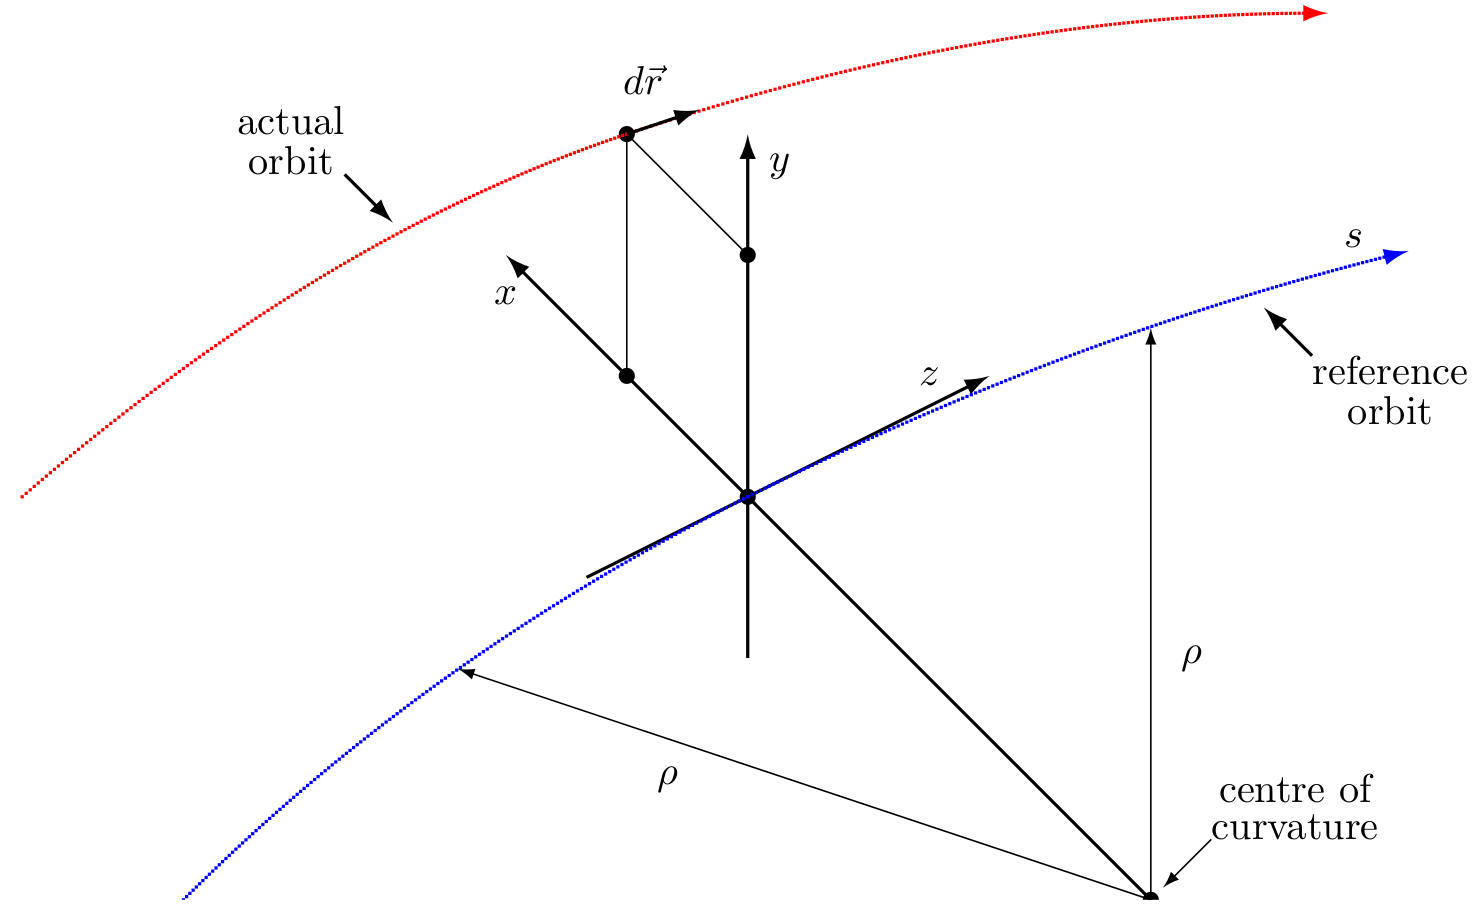
\includegraphics[scale=0.25]{figures/reference_system.png}
    % 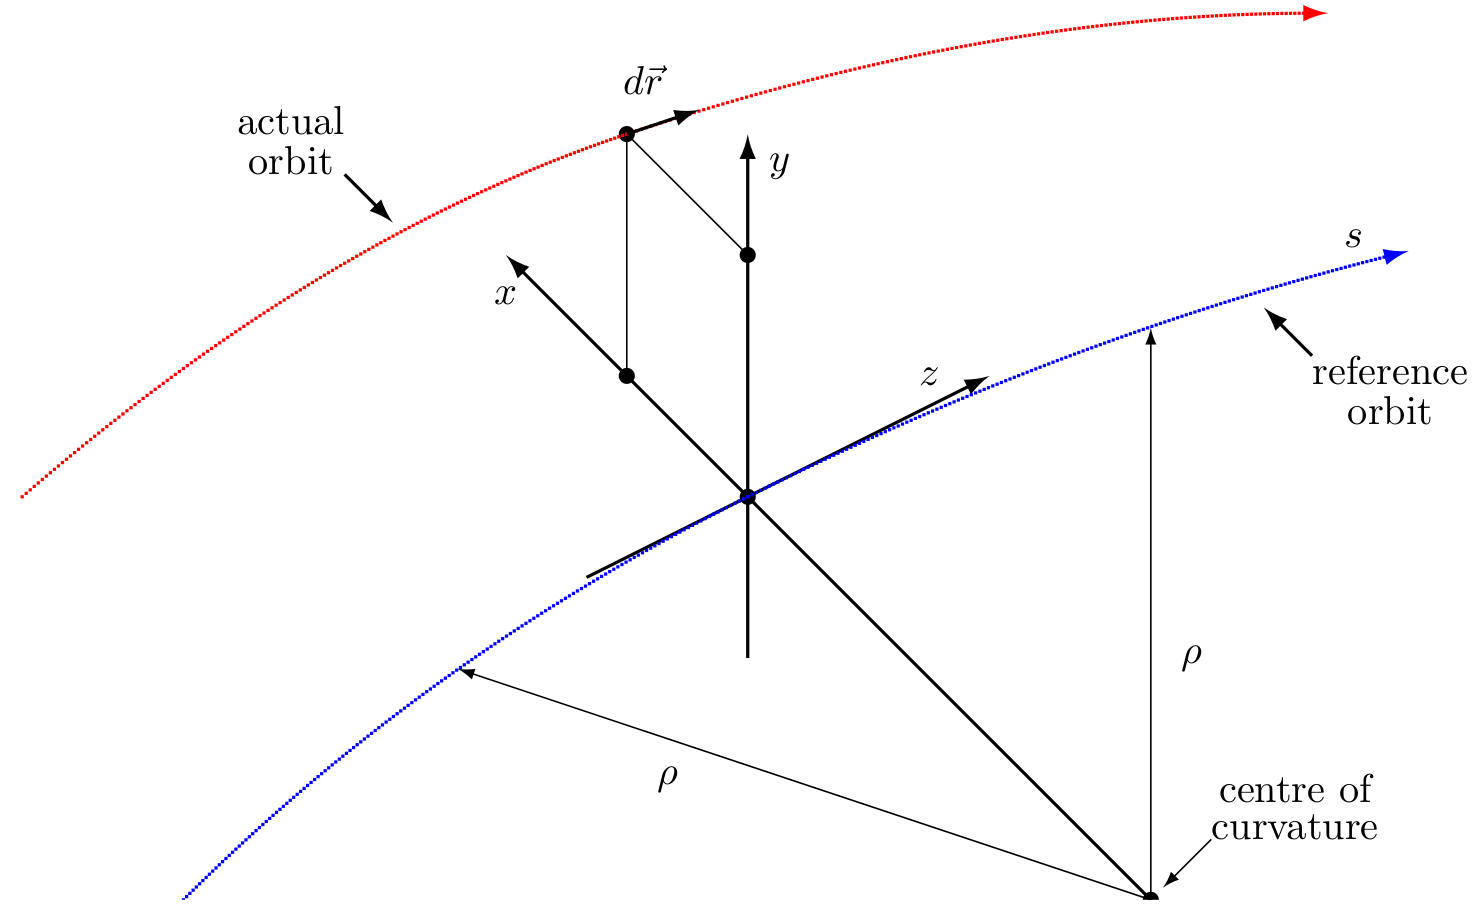
\includegraphics[width=\textwidth]{figures/reference_system.png}
    \caption{Coordinate system used in storage rings~\cite{madx}.}
    \label{syst}
\end{figure}

Electrons in a storage ring are in the ultra-relativistic regime, where $E \approx pc$ and the major contribution to the total momentum is longitudinal $p = \sqrt{p_s^2 + p_x^2 + p_y^2} \approx p_s$. It is assumed that transverse displacements $(x, y)$ of these electrons to the reference orbit are small, then the ratios $p_x/p$ and $p_y/p$ are small as well and they can be related to geometric quantities, namely angular deviations:
\begin{align*}
    x' &= \frac{\dif x}{\dif s} \approx \frac{p_x}{p}, \\
    y' &= \frac{\dif y}{\dif s} \approx \frac{p_y}{p}.
\end{align*}

The approximations made above are called paraxial. The coordinates $(x, x', y, y')$ defines a four dimensional (4D) phase space, where the transverse dynamics is described. Note that the displacements are functions of the longitudinal $s$ coordinate, replacing the time $t$ that is commonly used to describe the dynamics of a system. This substitution is convenient since the $s$ coordinate is periodic for a storage ring and the transverse coordinates derivatives can be interpreted geometrically.

To describe the longitudinal dynamics, one can define two more coordinates. The first is the difference of longitudinal position $s(t)$ of a generic electron relative to the position $s_{\mathrm{sync}}(t)$ of the synchronous electron:
\begin{equation}
    z(t) := s_{\mathrm{sync}}(t) - s(t).
\end{equation}

The variable $t$ represents the wall-clock time. The coordinate $z$ can be used in time units as well, represented by $\tau$ and the conversion is made by $\tau(t) = z(t)/c$. 

For the last coordinate it is used the electron relative momentum deviation from the nominal momentum, which is also typically small:
\begin{equation}
    \delta := \frac{p - p_0}{p_0} \approx \frac{E - E_0}{E_0},
\end{equation}
where the approximation follows from $E \approx pc$.

Finally, $(x, x', y, y', z, \delta)$ defines a six dimensional (6D) phase space where the transverse and longitudinal dynamics of the electrons in a storage ring can be studied.
\section{Transverse Dynamics}\label{tranverse}
The transverse dynamics describes the motion of the electrons in the 4D phase space $(x, x', y, y')$. In general, the typical time scale of the longitudinal dynamics is much larger than the transverse time scale and the two dynamics can be treated independently. This is called the adiabatic approximation and is a good approximation to describe the transverse motion in storage rings. In Sirius storage ring, while it takes around 200 turns to the electron perform one complete energy oscillation, in just one turn the same electron completes 49 and 14 oscillations in $x$ and $y$ planes, respectively.

% In the present section the linear transverse dynamics for a single electron in a storage ring is reported and the next one concerns its longitudinal dynamics.
\subsection{Betatron Oscillations}
A simpler version of a magnetic lattice is composed by dipoles and quadrupoles only. The dipoles bends the electrons path around the ring and defines an ideal orbit. The dipole field can be seen as the zero-order expansion of the lattice magnetic fields. The next terms of the expansion are field gradients, mainly related to the quadrupoles. This setup composes the linear magnetic lattice, where the magnetic field expansion is up to first order.

Assuming this linear approximation and that the transverse directions are independent, i.e., there is no transverse coupling terms, the Hamiltonian of an electron in the storage ring is \footnote{The approximated transverse Hamiltonian is obtained from the Hamiltonian of a relativistic charged particle on magnetic fields: $H = q\phi + c\sqrt{m^2c^2 + \left(\vec{p} - q\vec{A}\right) }$.}:
\begin{equation}
    H \approx \dfrac{{x'}^2}{2} + \dfrac{{y'}^2}{2} + \left(K(s)- G^{2}(s)\right)\dfrac{{x}^2}{2} - K(s) \frac{y^2}{2} - G(s) x \delta.
    \label{transv_hamilton}
\end{equation}

$G(s)$ is called curvature function and $K(s)$ is the focusing function, with the following expressions:
\begin{align}
    G(s) &= \dfrac{1}{\rho(s)} = \dfrac{e}{p_0}B(s), \\
    K(s) &= \dfrac{e}{p_0}\left.\dfrac{\partial B(s)}{\partial x}\right|_{y=0},
\end{align}
where $p_0$ is the ideal electron momentum. The dipoles magnetic field $B(s)$ must in the vertical direction to deflect the electrons horizontally. Observe that the function $G(s)$ is the inverse of the radius of curvature of the electron path through the dipoles. $G(s)$ and $K(s)$ are defined by the magnetic lattice and they are called lattice functions. For a storage ring, these functions are periodic, i.e., $G(s) = G(s+L_0)$ and $K(s) = K(s+L_0)$, where $L_0$ is the storage ring circumference.

% The quantity $R = B(s)\rho(s) = \dfrac{p_0}{e} \approx \dfrac{E_0}{ec}$ is called magnetic rigidity and it is a property of the stored electron. For the Sirius storage ring the electron magnetic rigidity is approximately 10.

From the Hamiltonian in Eq.~\eqref{transv_hamilton}, the equations of motion are:
\begin{align}
    x'' + \left(K(s) - G^{2}(s)\right)x &= G(s) \delta, \\
    y'' - K(s)y &= 0.
\end{align}

From the adiabatic approximation, in this derivation it was considered that the energy deviation $\delta$ is constant during the transverse motion.

The equation of motion for the horizontal plane contains a non-homogeneous term $G(s)\delta$ due to the dependence of position with energy created at dipoles. This term couples the horizontal and longitudinal motions.

If we consider only the homogeneous part, the $x$ and $y$ equations can be cast in the same form:
\begin{equation}
u'' + K_u(s) u = 0,
\label{hill}
\end{equation}
where $u = x$ or $y$, $K_x(s) = K(s) - G^2(s)$ and $K_y(s) = -K(s)$. Note that $K_x \approx -K_y$ if we consider $G^2/K \ll 1$, which is a good approximation for strong-focusing magnetic lattices. This reflects the fact that a focusing quadrupole in $x$ plane is necessarily defocusing in the $y$ plane and vice-versa. 

The homogeneous Eq.~\eqref{hill} is called Hill equation, which is similar to a simple harmonic oscillator equation, except for the important fact that the term $K_u$ is $s-$dependent and periodic. The authors in~\cite{CourantSnyder1958} proposed a pseudo-harmonic solution for the Hill equation:
\begin{equation}
    u_{\beta}(s) = \sqrt{2 J_u \beta_u (s)} \cos \left(\varphi_u(s) - \phi_u\right).
    \label{eq:beta_oscillation}
\end{equation}

This solution describes the so-called betatron oscillations. $\beta_u(s)$ is called betatron function and $\varphi_u(s)$ is the betatron phase advance. Inserting this solution in the Hill equation, it is obtained that the $\beta_u(s)$ must satisfy the following differential equation:
\begin{equation}
    \dfrac{1}{2}\beta_u {\beta''_u} -  \left(\dfrac{\beta'_u}{2}\right)^2 + K_u(s) \beta^2_u = 1,
    \label{beta_equation}
\end{equation}
and also that the betatron function and phase advance are related by
\begin{equation}
\varphi_u(s) = \int_{0}^{s} \dfrac{1}{\beta_u(\bar{s})} \dif \bar{s}.
\end{equation}

In storage rings, the betatron function is a periodic solution for Eq.~\eqref{beta_equation}.

The parameters $J_u$ and $\phi_u$ are constants defined by the electron initial conditions. One can show that the constant $J_u$ is written in terms of $(u, u')$ by
\begin{equation}
    2J_u = \gamma_u u^2 + 2 \alpha_u u u' + \beta_u {u'}^2,
    \label{invariant}
\end{equation}
for every longitudinal position $s$ and using the identities $\alpha_u(s) = -\beta_u'(s)/2$ and $\gamma_u(s) = (1 + \alpha_u^2(s))/\beta_u(s)$. These three functions $\left\{\alpha_u(s), \beta_u(s), \gamma_u(s)\right\}$ are called Twiss functions and depends only on the magnetic lattice.

In Eq.~\eqref{invariant} it is shown that, for each position $s$, the betatron oscillations performed by the electrons in the storage ring over the turns draw a ellipse in the phase space $(u, u')$. The ellipse shape varies with the longitudinal position $s$, however the ellipse area is constant for every $s$. Since the assumptions made so far allow us to consider the system as conservative, the ellipse area invariance in phase space can also be obtained from Liouville theorem. From Eq.~\eqref{invariant}, the ellipse area is $A_u = 2 \pi J_u$, following that $J_u$ is a invariant of motion. It is also possible to obtain this result applying the canonical transformation of action-angle variables in the Hamiltonian~\eqref{transv_hamilton}, identifying the action with $J_u$ (in this case, it is an invariant by construction), and the phase variable with $\varphi_u$.

Once these concepts are presented, we define the particle emittance as $\varepsilon_u = 2J_u$. In this way, the particle emittance can be interpreted as the area of the ellipse that electron follows in the 4D phase space during betatron oscillations, divided by $\pi$:
\begin{equation}
    \varepsilon_u = \frac{A_u}{\pi}.
\end{equation}

As discussed, it follows that the particle emittance is a invariant for the betatron motion. From the ellipse equation analysis, the maximum values for $u$ and $u'$ are:
\begin{align}
    u_{\beta, \mathrm{max}}(s) &= \sqrt{\varepsilon_u \beta_u(s)}, \\
    {u}_{\beta, \mathrm{max}}'(s) &= \sqrt{\varepsilon_u \gamma_u(s)}.
\end{align}

In a storage ring, the betatron phase advance accumulated over one turn is related to the number of betatron oscillations completed by the electrons. This number is called the tune of the machine, given by
\begin{equation}
    \nu_u = \dfrac{1}{2\pi} \oint \dfrac{1}{\beta_u({s})} \dif {s},
\end{equation}
where the closed integral represents an integration where the lower limit is an arbitrary $s$ and the upper limit is $s + L_0$, closing one turn around the ring.

The tune has a integer part (the number of complete betatron oscillations over one turn) and a fractional part. Because of this fractional part the values of $(x, x', y, y')$ at some $s$ may be different for each turn. The betraton oscillations peaks and valleys are $\pm \sqrt{\varepsilon_u \beta_u(s)}$. Therefore, the emittance $\varepsilon_u$ and the $\beta_u(s)$ function defines the envelope of the betatron oscillations. The importance of the betatron function will be further discussed throughout this work.

The tune fractional part is closely related to resonances. If the fractional part is zero, i.e., the tune is an integer number, in every turn the particles will have the same coordinates $(u, u')$ for every $s$. Then if there are dipolar field errors at the magnetic lattice, these errors will distort the electrons orbit in the same way at every turn, increasing the distortion amplitude and leading to electron losses. If the fractional part is $1/2$, the resonance is excited by quadrupolar field errors. Generally, there are resonances that can be excited if the tunes satisfy the relation
\begin{equation}
    m \nu_x + n \nu_y = r,
    \label{resonance}
\end{equation}
where $m, n, r \in \mathbb{Z}$. The order of resonance is $|m| + |n|$ and the resonance strength decays with the increase of its order, thus the lower order resonances are more harmful to the beam stability. The Eq.~\eqref{resonance} determines resonance lines in the space $(\nu_x, \nu_y)$ that must be avoided to prevent the electron beam from this type of instability. The tunes values must be carefully chosen for the machine operation point. The Sirius storage ring tunes are $\nu_x = 49.0962$ and $\nu_y=14.1520$.
\subsection{Dispersion function}
It can be seen from the radius of curvature created by the dipoles that an electron with energy deviation $\delta$ will be more deflected if $\delta < 0$ and less deflected if $\delta > 0$, compared to the on-energy electron with $\delta = 0$. Thus this energy difference is translated in different horizontal displacements. This effect is represented by the non-homogeneous term $G(s)\delta$ in the horizontal equation of motion, which couples longitudinal and horizontal motions.

The homogeneous equation was already solved in the last section, leading to betatron oscillations $x_{\beta}$. Therefore the general solution to the horizontal plane is a combination of $x_{\beta}$ and a particular solution for the non-homogeneous equation. As discussed, it is known that this particular solution must be a function of $s$ and $\delta$. From linearity with respect to energy deviations
\begin{equation}
    x(s, \delta) = x_{\delta}(s) = \eta(s) \delta,
\end{equation}
where the $s$-dependence is retained in the function $\eta(s)$, called dispersion function. Inserting the proposed solution in the differential equation, it is obtained that $\eta(s)$ must satisfy
\begin{equation}
    \eta'' + K_x(s)\eta = G(s).
    \label{eq:dispersion}
\end{equation}

For a periodic magnetic lattice as used in storage rings, $\eta(s)$ is a periodic solution to this differential equation.

We finally obtained the transverse displacements solutions to the equations of motion, where $x(s) = x_{\beta}(s) + x_{\delta} (s)$ and $y(s) = y_{\beta}(s)$. 

Imperfections such as magnet misalignment or construction errors can introduce horizontal dipolar and skew quadrupolar fields, generating a vertical dispersion function, i.e., a dependence on vertical position with energy as well. Nevertheless, in this case the steps made to obtain the solution for $x$ plane can be reproduced to obtain a equivalent solution to the $y$ plane. Moreover, typically it is desired to keep $\eta_y(s)$ as low as possible and there are some strategies to achieve this goal, which will be discussed in this work.
\section{Longitudinal dynamics}\label{longitudinal}
In the previous section it was considered that the electron energy remains constant during the transverse motion typical time scale, which is a good approximation. On the other hand, since electrons are charged particles and in a storage ring they are submitted to centripetal acceleration at dipoles and \gls{id}s, the so-called sychrotron radiation is generated and the electrons lose energy. The energy loss is then compensated by the accelerating fields contained in the \gls{rf} cavity. During this process the electron energy oscillates and this motion is known as synchrotron oscillations.
\subsection{Orbit Length}
To calculate the orbit length, one has to average the electron path over many turns. In this process the betatron oscillations occurs several times, adding and subtracting almost equally to the path length. Therefore the betatron motion does not contribute to the orbit length in first order. On the other hand, the horizontal energy-dependent term $x_{\delta}(s) = \eta(s) \delta$ has a significant contribution. 

The momentum compaction factor is a parameter that depends on the magnetic lattice and is fundamental to the longitudinal dynamics. It can be defined as:
\begin{equation}
    \alpha := \dfrac{1}{L_0}\oint G(s) \eta(s) \dif s,
\end{equation}
where $\alpha$ can be positive, negative or zero as well. 

The orbit length is related to the momentum deviation by:
\begin{equation}
    \frac{\Delta L}{L_0} = \alpha \dfrac{\Delta p}{p_0} = \alpha \delta.
    \label{orbitlen}
\end{equation}

Typically $\alpha > 0$ in synchrotrons. In this case, from Eq.~\eqref{orbitlen}, an electron with $\delta > 0$ is less deflected by the dipoles, following a path with greater radius, therefore greater length $\Delta L > 0$, as compared to the nominal orbit length $L_0$. The opposite happens for an electron with $\delta < 0$. 
% \begin{equation}
%     \frac{\Delta L}{L_0} = \left(\alpha - \dfrac{1}{(v/c)^2\gamma^2}\right) ,
%     \label{slip}
% \end{equation}
% where $\alpha$ is called the momentum compaction factor. The term $\alpha - \dfrac{1}{(v/c)^2\gamma^2}$ is known as slip factor and, for ultra-relativistic electrons, it is very close to $\alpha$. For example, on Sirius storage ring $\alpha = 1.6 \times 10^{-4}$, $v/c \approx 1$ and $\gamma = 5871$, so the difference between the slip factor and $\alpha$ is only $3 \times 10^{-8}$. Using $\delta \approx \dfrac{\Delta p}{p_0}$, the Eq.~\eqref{slip} is commonly written as:

% This type of closed integral around the ring is common during the derivation of lattice and beam parameters. There are five integrals, called synchrotron radiation integrals, that appears in the expressions of many parameters, so it is useful to label them. The first synchrotron integral is the one used to calculate the momentum compaction factor
% \begin{equation}
%     I_1 = \oint G(s) \eta(s) \dif s = \oint \dfrac{\eta(s)}{\rho(s)} \dif s.
% \end{equation}
% Then, the momentum compaction factor is written as $\alpha = I_1/L_0$.
\subsection{Synchrotron Oscillations}
% Energy oscillations are not directly explored in this work, however it was considered appropriated to include the basic ideas for the sake of completeness of the presented theory.
Consider the synchronous electron with the nominal energy $E_0$, following the ideal orbit through the storage ring. In each turn, this electron will radiate synchrotron light, losing the amount $U_0$ of energy. $U_0$ is typically much lower than the electron energy $E_0$. An electron with energy $E_0$ but not following the ideal orbit will perform several betatron oscillations in one turn and the transverse displacements will average to zero in first order. Hence, in this case, the energy loss per turn will be $U_0$ too. 

On the other hand, the energy loss per turn has a first order difference from $U_0$ for an electron with energy deviation $\delta$. This off-energy electron will follow an orbit displaced horizontally by $\eta(s)\delta$ and the electron will experience different fields along the ring. Furthermore, the energy loss depends on the electron energy by itself as well. On account of these two effects, the energy loss must be a function $U_{\mathrm{rad}}(\delta)$ satisfying $U(0) = U_0$. It is considered that $\delta \ll 1$ for electrons in a storage ring, so it is reasonable to keep only the linear part of $U_{\mathrm{rad}}(\delta)$:
\begin{equation}
    U_{\mathrm{rad}}(\delta) \approx U_0 + \dfrac{\dif U_{\mathrm{rad}}}{\dif \delta}\delta.
    \label{approx1}
\end{equation}

The energy gain process concerns the \gls{rf} accelerating system. The resonant cavity installed in the storage ring receives a RF signal, creating an oscillating electric field inside the cavity. This electric field has a longitudinal component that might accelerate the electrons and allow for the electrons energy recovery.

The electric field mentioned has a related time-dependent potential $V(t)$, which is the integrated electric field inside the cavity along the longitudinal direction. Since this potential is oscillating in time, the possible electron energy gain per turn is also time dependent. In order to keep the electron energy stable, the ideal electron energy balance must be zero, i.e., the energy gained by the RF cavity must always be $U_0$ at each turn. To achieve this, the ideal electron circular motion must be synchronized to the RF voltage oscillation and this is why ideal electrons are also called synchronous electrons. This equivalent to the requirement that the RF cavity potential oscillating frequency $f_{\mathrm{rf}}$ must be a multiple of the ideal electron revolution frequency $f_0$
\begin{equation}
    f_{\mathrm{rf}} = h f_0,
\end{equation}
where integer $h$ is called harmonic number.

We are interested in deviations from the synchronous electron, then the absolute time dependence of $V_{\mathrm{rf}}(t)$ can be replaced by the coordinate $\tau(t) = z(t)/c$ that is the relative difference to the ideal arrival time at the cavity. In this way, an electron energy gain is given by $eV_{\mathrm{rf}}(\tau)$ and for the ideal electron we require that $eV_{\mathrm{rf}}(0) = U_0$. Since the longitudinal displacements $\tau$ are small as well, we may expand in first order the energy gain:
\begin{equation}
    U_{\mathrm{rf}}(\tau) = eV_{\mathrm{rf}}(\tau) \approx U_0 + e\dfrac{\dif V_{\mathrm{rf}}}{\dif \tau}\tau.
    \label{approx2}
\end{equation}

Now we are ready to obtain the differential equation for the longitudinal motion. Observe that from Eq.~\eqref{orbitlen} the orbit length (and the revolution time) depends on the energy deviation $\delta$. Let the sub-index $n$ denote the turn number. In successive turns the relative position $z(t)$ changes by $\Delta z = z_{n+1} - z_n = \alpha\delta_n L_0$. Converting it to time variables, then $\Delta \tau = \alpha \delta_n T_0$, where $T_0$ is the revolution period. As mentioned, the longitudinal dynamics time scale is much greater than the time involved in one turn, then longitudinal changes in consecutive turns divided by the revolution time $T_0$ can be regarded as derivatives. Hence
\begin{equation}
    \dfrac{\dif \tau}{\dif t} = \alpha \delta.
    \label{long_diff1}
\end{equation}

From the electron energy balance $\Delta E = E_{n+1} - E_n = eV(\tau_n) - U_{\mathrm{rad}}(\delta_n)$. Dividing by $T_0$ and $E_0$ we obtain:
\begin{equation}
    \dfrac{\dif \delta}{\dif t} = \dfrac{eV_{\mathrm{rf}}(\tau) - U_{\mathrm{rad}}(\delta)}{E_0 T_0}.
    \label{long_diff2}.
\end{equation}

The two coupled differential equations~\eqref{long_diff1} and~\eqref{long_diff2} describes the longitudinal dynamics in the phase space $(\tau, \delta)$.

With the linear approximations made in equations~\eqref{approx1} and~\eqref{approx2}, the differential equations can be cast in the following form:
\begin{equation}
    \Ddot{v} + 2\alpha_{z} \dot{v} + \omega_{z}^2 v = 0,
    \label{damped}
\end{equation}
where $v=\tau$ or $\delta$ and the dot represents the time derivative. The Eq.~\eqref{damped} describes a damped harmonic oscillator, with frequency $\omega_z = \sqrt{\dfrac{\alpha e}{E_0 T_0} \dfrac{\dif V_{\mathrm{rf}}}{\dif \tau}}$, called synchrotron frequency. The term $\alpha_z = \dfrac{1}{2T_0} \dfrac{\dif U_{\mathrm{rad}}}{\dif \delta}$ is positive, represents the effect of radiation damping and it is typically small. 

In the small oscillation limit, the phase-space trajectories are ellipses with decreasing radius towards $\tau = \delta = 0$. In the general case of large oscillations, the longitudinal dynamics is not equivalent to a damped oscillator anymore and the dynamics is non-linear. The electrons trajectories in phase space are divided in two classes: 1) closed, limited and stable and 2) open, unlimited and unstable. The stable regions in the phase space are called \gls{rf} buckets and a separatrix delimits the stable from the unstable region, where the limit is the stable trajectory with largest amplitudes.

It is important to observe that to keep electrons oscillating longitudinally, it is required that $\left.\dfrac{\dif V_{\mathrm{rf}}}{\dif \tau}\right|_{\tau = 0} > 0$, otherwise the synchrotron frequency would be an imaginary number and the motion would be unstable. Note that while the ``restoring force'' for the betatron oscillation comes from the focusing function (basically the field gradients), the equivalent for the synchrotron oscillations comes from the \gls{rf} potential derivative.

The typical \gls{rf} potential is sinusoidal $V_{\mathrm{rf}}(\tau) = \hat{V}_{\mathrm{rf}} \sin \left(\omega_{\mathrm{rf}}\tau + \phi_s\right)$ where $\hat{V}_{\mathrm{rf}}$ is the peak \gls{rf} potential. From the energy balance $eV_{\mathrm{rf}}(0) = U_0$ we obtain that $\sin(\phi_s) = U_0/e\hat{V}_{\mathrm{rf}}$ and $\phi_s$ is called, as expected, the synchronous phase. During the \gls{rf} signal tuning one needs to adjust the \gls{rf} phase signal in order to find the synchronous phase which allows for electrons storage.

Since $\omega_{\mathrm{rf}} = h \omega_0$, where $\omega_0$ is the angular revolution frequency, there are $2h$ occurrences of $eV_{\mathrm{rf}}(0) = U_0$ during one revolution period but only in half of them the stability condition $\left.\dfrac{\dif V_{\mathrm{rf}}}{\dif \tau}\right|_{\tau = 0} > 0$ is satisfied. Because of that there are $h$ \gls{rf} buckets in the longitudinal phase space, where electrons can be stored in bunches. For the Sirius storage ring, it is possible to accumulate electrons in 864 bunches.
\subsection{Phase Stability}
The principle of phase stability is a fundamental concept to the realization of synchrotron light sources. It establishes a mechanism that guarantees that electrons with energy or longitudinal phase deviations will be forced towards the synchronous condition.

It will be helpful to convert the Eq.~\eqref{orbitlen} in terms of revolution times, writing as $\Delta T/T_0 = \alpha \delta$. Suppose an electron with energy deviation $\delta > 0$ in a storage ring, then it will take more time to this electron perform one turn, to reach the \gls{rf} cavity and from the convention used to the coordinate definition, $\tau < 0$ to this electron. Since the \gls{rf} potential derivative must be positive at $\tau = 0$, the energy gain $U_{\mathrm{rf}}$ for $\tau < 0$ is less than $U_0$; moreover, $U_{\mathrm{rad}} > U_0$ for electrons with $\delta > 0$. Thus, the energy balance for this electron will be negative, leading it to lower values of $\delta$ and also $\tau$.

The analysis is basically the same for electrons initially with $\delta < 0$. These electrons will perform each turn faster than the synchronous electron does, having $\tau > 0$ and gaining more energy from the cavity than it is lost by radiation. This positive energy balance will increase the values of $\delta$ and $\tau$.

The phase stability principle guarantees that the electrons will oscillate around the longitudinal fixed point $(\tau = 0, \delta = 0)$. The radiation damping effect says that the longitudinal deviations might be eventually damped to this fixed point. On the counterpart, the quantum nature of radiation emission produces an excitation effect and the balance between damping and excitation creates an equilibrium configuration.

Since the synchronous condition must be satisfied, from Eq.~\eqref{orbitlen} it is obtained that:
\begin{equation}
    \dfrac{\Delta f_{\mathrm{rf}}}{f_{\mathrm{rf}}} = -\alpha \delta.
    \label{eq:delta_freq}
\end{equation}

From this equation it can be seen that a change in the \gls{rf} frequency forces the electrons to follow an off-energy orbit. In the \gls{rf} tuning, one must adjust the \gls{rf} frequency to match the condition $\delta = 0$ and this can be performed by making the horizontal orbit average go to zero, since the orbit displacement is related to the energy deviation by the dispersion function.

Beyond the importance of phase stability in storage rings, it is also this principle that allows for increasing the electron energy in synchrotrons. Increasing the magnetic fields will force the electrons to reach new synchronous conditions related to higher energies. To achieve that, the electrons must gain more energy from the \gls{rf} cavity and the phase stability principle drives this process automatically. In the Sirius booster, the electron energy ramp is performed from \SI{150}{\mega \electronvolt} to \SI{3}{\giga \electronvolt}.
% \section{Equilibrium Parameters}\label{equilibrium}
% Two opposite effects acts on the electron beam to result in equilibrium parameters: the radiation damping and the quantum excitation. The radiation emission is a quantum process, where the photon emissions occur randomly and are statistically independents. The radiation emission provides sudden energy jumps in the electron energy and excites both betatron and synchrotron oscillations.

% For the synchrotron oscillations the excitation is obvious. Each photon emitted produces a negative energy deviation in the electron, so it increases the energy oscillation amplitude. In the transverse coordinates, this negative energy deviation produces an additional orbit displacement by the means of dispersion function, then the electron will perform betatron oscillations around this new off-energy orbit, which might have greater amplitudes than before the photon emission, depending on the betatron phase at the emission position.

% It was shown in Section \ref{longitudinal} that the linear dependence of the energy loss by radiation on the electron energy deviation, the positive derivative $\dfrac{\dif U_{\mathrm{rad}}}{\dif \delta}$, produces a damping term in synchrotron oscillations: as the electron energy is higher it radiates more energy. The damping of betatron oscillations comes from the manner that the \gls{rf} cavity field accelerates the electrons and replaces its energy. The radiation emission reduces the momentum magnitude, $p = \sqrt{p_s
% ^2+ p_x^2 +p_y^2}$, but does not change the vector direction. Moreover, the longitudinal electric fields in the \gls{rf} cavity adds only to the longitudinal component of the momentum. Therefore, after the energy loss and gain processes, the momentum magnitude is the same but the transverse components $p_x$ and $p_y$ are reduced and the longitudinal component $p_s$ is increased, leading to the damping of the transverse motion.
% \subsection{Emittance}
% The classical radiation power emitted for a relativist electron with energy $E$ in a magnetic field $B$ perpendicular to the electron path is given by~\cite{jackson}:
% \begin{equation}
%     P_{\gamma} = \dfrac{e^2c^3}{2\pi} C_{\gamma} E^2 B^2,
% \end{equation}
% where the constant $C_{\gamma} = \dfrac{4 \pi r_e}{3 (mc^2)^3} \approx \SI{8.85e-5}{\metre {\giga \electronvolt}^{-3}}$ and $r_e$ is classical electron radius. Writing the radiation power in terms of the local curvature radius:
% \begin{equation}
%     P_{\gamma} = \dfrac{cC_{\gamma}}{2\pi} \dfrac{E^4}{\rho^2}.
% \end{equation}

% The total energy radiated per turn for electrons with nominal energy can be obtained by integrating the radiation power in one revolution period. Since $s = ct$, equivalently one can change the integration variable to $s$ and substitute the local radius $\rho$ by the curvature function $G(s)$:
% \begin{equation}
% U_0 = \dfrac{C_{\gamma}E_0^4}{2\pi} \oint G^{2}(s) \dif s.    
% \end{equation}

% Here we define the second synchrotron radiation integral:
% \begin{equation}
%     I_2 = \oint G^{2}(s) \dif s = \oint \dfrac{1}{\rho^2(s)} \dif s,
% \end{equation}
% then the energy loss per turn is written as $U_0 = C_{\gamma}E_0^4 I_2/2\pi$.

% The origin of the other three synchrotron radiation integrals are more involved to be explained. Since it is not in the dissertation's scope, they will just be defined with their related parameters. 
% \begin{align}
%     I_3 &= \oint |G(s)|^3 \dif s = \oint \dfrac{1}{|\rho(s)|^3} \dif s, \\
%     I_4 &= \oint \eta(s) G(s) \left(G^2(s) + 2 K(s)\right) \dif s, \\
%     I_5 &= \oint \mathcal{H}(\eta, \eta') |G(s)|^3 \dif s,
%     \label{eq:integral5}
% \end{align}
% where $\mathcal{H}$ is a functional given by
% \begin{equation}
%     \mathcal{H}(\eta, \eta') = \gamma \eta^2 + 2 \alpha \eta \eta' + \beta {\eta'}^2.
% \end{equation}

% From the analysis of the radiation damping effects on the transverse and longitudinal dynamics, one can obtain the damping rates for each oscillation. These damping rates are related to the so-called damping partition numbers, given by\footnote{Historically it was also chosen the letter $J$ to represent the damping partition numbers, care must be taken to do not confound it with the action variables.}
% \begin{equation}
%     J_x = 1 - \dfrac{I_4}{I_2}, \hspace{0.5cm} J_y = 1, \hspace{0.5cm} J_{\delta} = 2 + \dfrac{I_4}{I_2}.
% \end{equation}

% Note that $J_x + J_y + J_{\delta} = 4$, which is a general result obtained from the Robinson Theorem~\cite{Robinson1958}. The value $J_y = 1$ reflects the assumption of zero vertical dispersion. In the presence of vertical dispersion, the first, fourth and fifth synchrotron integrals are divided in two components: $I_{i, x}$ and $I_{i, y}$, where $i = 1, 4, 5$. In this case the damping partition numbers are: 
% \begin{equation*}
%     J_x = 1 - \dfrac{I_{4,x}}{I_2}, \hspace{0.5cm} J_y = 1 - \dfrac{I_{4,y}}{I_2}, \hspace{0.5cm} J_{\delta} = 2 + \dfrac{I_{4,x} + I_{4,y}}{I_2}.
% \end{equation*}

% The damping rates for each coordinate can be obtained by $\alpha_{\mu} = J_{\mu} \alpha_0$, where $\mu = x, y$ or $\delta$ and $\alpha_0 = \dfrac{U_0}{2E_0T_0}$. The damping times are simply $\tau_{\mu} = 1/\alpha_{\mu}$.

% Including the damping and excitation effects, the natural equilibrium transverse emittance of the electron beam is:
% \begin{equation}
%     \varepsilon_0 = C_q \gamma^2 \dfrac{I_5}{J_x I_2},
%     \label{eq:emittance}
% \end{equation}
% where $C_q = \dfrac{55}{32 \sqrt{3}}\dfrac{\hbar}{mc} \approx \SI{3.84e-13}{\metre}$ and $J_x$ is the horizontal damping partition number.

% From the Eq.~\eqref{eq:emittance} and the definition of the integral $I_5$ in Eq.~\eqref{eq:integral5}, it is evident that the equilibrium emittance depends strongly on the dispersion function at the dipoles. Therefore, minimizing the values of the functional $\mathcal{H}(\eta, \eta')$ at the dipoles is one approach that can be taken in order to minimize the natural emittance for a storage ring. One would expect this intuitively knowing that the photon emission occurs at the dipoles, then if the dispersion is as low as possible at these magnets, the quantum excitation contribution to the transverse action may be reduced.

% Ideally the vertical dispersion function is zero and the horizontal and vertical dynamics are uncoupled, then the horizontal emittance is equal to the natural emittance and the vertical emittance is zero. If there are some field or rotation errors in the magnets, the betatron oscillations might be coupled. In this case of betatron coupling, the horizontal emittance is shared with the vertical emittance. One of the definitions of the betatron coupling is the emittance ratio $\kappa = \varepsilon_y/\varepsilon_x$. The nominal emittance is $\varepsilon_0 = \varepsilon_x + \varepsilon_y$ and the transverse emittances are
% \begin{align}
%     \varepsilon_x &= \dfrac{1}{1 + \kappa}\varepsilon_0, \\
%     \varepsilon_y &= \dfrac{\kappa}{1 + \kappa}\varepsilon_0.
% \end{align}

% If there is a considerable vertical dispersion function in the storage ring, there will be a vertical emittance even if there is no betatron coupling between the transverse planes $(\kappa = 0)$ and the natural emittance will be increased. In this case, as already mentioned, there are two integrals $I_{5, x}$ and $I_{5, y}$, each one calculated with the respective dispersion function in the functional $\mathcal{H}$. Thus, the corresponding emittances are $\varepsilon_u = C_q \gamma^2 \dfrac{I_{5, u}}{J_u I_2}$, where $u=x$ or $y$ and the natural emittance is the sum $\varepsilon_0 = \varepsilon_x + \varepsilon_y$.
% \subsection{Beam Size and Divergence}
% The equilibrium transverse beam dimensions are also a result from the balance between the excitation and damping processes. The transverse displacements for the particles in the beam can be regarded also as gaussian distributions, so their~\gls{std} can be used to characterize the beam dimensions. From the betatron oscillation expression in Eq.~\eqref{eq:beta_oscillation} and their derivatives one can calculate:
% \begin{align}
%     \langle u_{\beta}^2 \rangle &= \beta_u(s) \langle J_u \rangle,  \\
%     % \langle u_{\beta} {u}_{\beta}' \rangle &= -\alpha_u(s) \langle J_u \rangle,  \\
%     \langle {u'_{\beta}}^{2} \rangle &= \gamma_u(s) \langle J_u \rangle,
% \end{align}
% where $\langle \cdot \rangle$ denotes the average performed on an ensemble of particles at a position $s$. One can identify that the beam emittance is the average of the particle actions, so $\varepsilon_u = \langle J_u \rangle$. Since the betatron oscillations occurs around the origin, $\langle u_{\beta}\rangle = \langle u'_{\beta}\rangle = 0$. 

% The off-energy displacements $\eta(s)\delta$ also play a role in the beam dimensions. The energy deviations for the particles is also approximately a gaussian distribution centered at zero (so $\langle \delta \rangle = 0$) and its~\gls{std} is called beam energy spread:
% \begin{equation}
%     \sigma^2_{\delta} = \langle \delta ^2\rangle = C_q \gamma^2\dfrac{I_3}{J_{\delta}I_2}.
% \end{equation}

% Thus, the transverse beam size and divergence can be obtained from $\sigma^2_u = \langle\left(u_\beta + \eta_u \delta\right)^2\rangle$ and $\sigma^2_{u'} = \langle\left(u'_\beta + \eta'_u \delta\right)^2\rangle$, resulting in
% \begin{align}
%  \sigma^2_u(s) &= \beta_u (s) \varepsilon_u + \left(\eta_u(s) \sigma_{\delta}\right)^2, \\
%  \sigma^2_{u'}(s) &= \gamma_u (s) \varepsilon_u + \left(\eta_{u}'(s) \sigma_{\delta}\right)^2.
% \end{align}

% From the equations above it can be seen that to obtain an electron beam with small transverse size and divergence as a source for synchrotron light in a specific longitudinal position $s$, it is required a combination of small transverse emittances (which are global parameters) and low values of betatron and dispersion functions at the location $s$.

% Finally, the longitudinal beam size, named bunch length, is given by
% \begin{equation}
%     \sigma_{z} = \dfrac{\alpha}{\omega_z} \sigma_{\delta},
% \end{equation}
% remembering that $\alpha$ is the momentum compaction factor and $\omega_z$ the synchrotron frequency. The bunch length is a very important parameter to study of effects that involves the electron density in a bunch, such as the scattering between these electrons, which is responsible for the main contribution to the beam lifetime, the so-called Touschek lifetime~\cite{touschek}.
\section{Perturbations}\label{perturbations}
The effects of magnets and field errors in the electron beam can be minimized with increasingly advanced techniques for magnets construction and alignment. Nevertheless, the errors are impossible to be completely eliminated in practice. Furthermore, the magnets parameters are measured by bench devices that are less sensible to the errors than the electron beam. Hence, deviations from ideal conditions must be considered in the accelerator physics studies in order to develop methods for their diagnostics and corrections.

In this section we will present the perturbations on the electron beam properties caused by low-order errors that are found in storage rings. 
\subsection{Orbit}\label{subset:orbit}
The first natural error type to be studied is the dipolar. The presence of these dipolar errors disturbs the closed orbit for the electron motion. Depending on the distribution and the magnitude of these errors, a closed orbit solution may not even exist, then it would be impossible to keep electrons in stable conditions in the storage ring without corrections. Typically, even considering that all the specifications regarding the magnets fabrication and alignment were met, the dipolar errors might provide a closed orbit solution with large distortions around the ring. Despite this, the orbit distortions can be measured by the \gls{bpm}s and corrected with dipolar correctors (or steering magnets), forcing the disturbed closed orbit to approach the ideal closed orbit.

The typical sources of dipolar errors are:
\begin{itemize}
    \item Dipolar fields from transverse alignment errors in quadrupoles. An electron with the deviation $x$ passing through a focusing quadrupole perfectly aligned to the reference orbit will receive a force $-Kx$ in the horizontal plane. If the quadrupole center is misplaced from the center by $x_0$, the focusing force will be $-K(x - x_0)$, therefore the misalignment introduces an additional dipolar term $K x_0$ every time the elecrons pass through this quadrupole. This is called feed-down effect\footnote{The Appendix~\ref{appendix:feed-down} is dedicated to brief discussions and derivations related to this effect.}, in which alignment errors in $n$-order fields will produce $(n-1)$-order fields contributions.
    \item Differences between ideal and real dipolar fields in the dipoles magnets, due to fabrication errors or remnant fields. In the case of electromagnets, the excitation curve that relates the applied current on the power supply and the magnetic field in the magnet must be well calibrated, otherwise the actual field in the magnets will differ from the expected. 
    \item Horizontal dipolar fields, which should be ideally zero, due to rotation errors in the dipoles magnets.
    \item Spurious magnetic sources along the ring, such as ion pumps, leak fields from injection pulsed magnets, etc.
\end{itemize}
We will study how a dipolar error $\Delta G_u$ (where $u=x, y$), localized in a small longitudinal region $\Delta s$, affects the closed orbit solution. The additional term $\Delta G_u$ can be regarded as a perturbation in the Hamiltonian~\eqref{transv_hamilton} for the transverse dynamics. An approximation can be made to consider the dipolar error as a localized ``kick'': 
\begin{equation*}
    \lim_{\Delta s \rightarrow 0}\Delta G_u(s)\Delta s = \theta_{s_0} \delta(s - s_0),
\end{equation*}
where $\delta(s-s_0)$ is the Dirac delta distribution centered at $s_0$, so in this way the quantity $\Delta G_u(s)\Delta s$ is finite in the limit $\Delta s \rightarrow 0$. This dipolar kick will add a sudden change in the angle of the electron trajectory when it reaches $s_0$, given by:
\begin{align*}
    \Delta u'(s_0) &= \Delta G_v(s) \Delta s \\
    &= -\oint \theta_{s_0} \delta(s - s_0) \dif s = -\theta_{s_0}.
\end{align*}

If the dipolar field error is vertical, $v=y$, the angle change is horizontal, $u=x$ and the dipolar kick is also named as horizontal. If the field error is horizontal, $v=x$, the angle change is vertical, $u=y$ and the kick is called vertical. The sign follows from angle coordinate definition, if $\Delta G_y > 0$ then $\Delta x' < 0$ and if $\Delta G_x > 0$, then $\Delta y' > 0$.

The angle change will produce betatron oscillations in the electron motion, reaching the dipolar error in each turn with different position and angle conditions. After some time, the transverse motion will be damped to a distorted closed orbit. 

In the presence of this dipolar kick, the transverse equations of motion  are:
\begin{align}
    x'' + K_x(s)x &= G_y(s) \delta - \Delta G_y(s), \\
    y'' + K_y(s)y &= \Delta G_x(s).
\end{align}

Remember that $u'' = \frac{\Delta u'}{\Delta s}$, then writing the above equations as $\Delta u' + K_u(s) u \Delta s = \Delta G_v(s) \Delta s$ and taking the limit $\Delta s \rightarrow 0$, $\Delta u' = \theta^{u}_{s_0}$ is recovered. 

With the kick approximation, the dipolar error can be viewed as an impulse term in the linear differential equations for the transverse motion. Hence, the theory of Green's function can be applied. The solution obtained from this analysis is~\cite{wiedemann2007physics}
\begin{equation}
    \Delta u(s) = \dfrac{\sqrt{\beta_{u}(s)\beta_{u}(s_0)}}{2\sin\left(\pi\nu_{u}\right)} \theta_{s_0}^{u} \cos\left( |\varphi_{u}(s) - \varphi_{u}(s_0)| - \pi\nu_{u} \right),
\end{equation}
and this is the orbit distortion for a dipolar error localized in the position $s_0$. The generalization for a distribution of errors $\theta_u(s)$ is quite direct:
\begin{equation}
    \Delta u(s) = \oint \dfrac{\sqrt{\beta_{u}(s)\beta_{u}(\bar{s})}}{2\sin\left(\pi\nu_{u}\right)} \theta_{u}(\bar{s}) \cos\left( |\varphi_{u}(s) - \varphi_{u}(\bar{s})| - \pi\nu_{u} \right) \dif \bar{s}.
    \label{eq:orbit_distortion}
\end{equation}

Note that the orbit distortion diverges if the tune fractional part is an integer. Here the connection between dipolar fields errors and integer resonances becomes explicit. Moreover, it is very important to point out that the orbit distortion depends on the betatron functions and the betatron phase advances, i.e., it depends on the optics parameters of the magnetic lattice.
\subsection{Optics}\label{subsec:optics}
Quadrupolar (or gradient) errors disturbs the focusing functions in the magnetic lattice, therefore perturbs the storage ring linear optics . The typical sources of quadrupolar errors are:
\begin{itemize}
    \item Differences between ideal and real gradient fields in the quadrupoles magnets, due to fabrication errors or remnant fields. The excitation curve must be well calibrated too, otherwise the actual field in the magnets will differ from the expected. 
    \item Gradient fields in dipoles magnets that are not expected in the magnets field characterization.
    \item Feed-down effects from horizontal alignment errors in sextupoles magnets. An electron with the deviation $x$ passing through a focusing sextupole perfectly aligned to the reference orbit will receive a force $-Sx^2$ in the horizontal plane. If the sextupole center is misplaced from the center by $x_0$, the force will be $-S(x - x_0)^2$, therefore the misalignment introduces an additional horizontal focusing term $ Sx_0 x$, where the focusing strength is given by $Sx_0$, and a dipolar term $-S x_0^2$, which will influence the electrons every time they pass through this sextupole.
\end{itemize}

A gradient error $\Delta K_u$ (where $u=x, y$), localized in a small longitudinal region $\Delta s$ will change the conditions in the differential Eq.~\eqref{beta_equation} that the betatron function must satisfy. Therefore this error will disturb the betatron function solution, consequently the betatron phase advance and finally the betatron tunes.

An approximation can be made to consider the single gradient error as a thin lens. The focal length added in this case is $1/f_u = \Delta K_u \Delta s$. If the gradient error is on a quadrupole with length $L$, the focal length is the obtained from the integrated field along the quadrupole, $1/f_u = \Delta K_u L$. With this approximation the gradient error effect can be regarded as an impulse $\Delta K_u(s) = \Delta K_u \delta(s-s_0)$ located at $s_0$.

Assuming the error $\Delta K_u$ is small, then only first order terms might be kept. The correspondent change in the betatron tunes for a integrated gradient error $\Delta K_u L$ located at $s_0$ can be obtained as
\begin{equation}
    \Delta \nu_u = \dfrac{1}{4 \pi} \beta_u (s_0) \Delta K_u L.
\end{equation}

For a quadrupole, $\Delta K_x = - \Delta K_y$, then a positive error in the focusing strength will increase $\nu_x$ and decrease $\nu_y$. Note that the tune change depends on the non-perturbed betatron function value at the error location.

For a general gradient error distribution around the ring, the tune change is:
\begin{equation}
    \Delta \nu_u = \dfrac{1}{4 \pi} \oint \beta_u ({s}) \Delta K_u ({s})\dif {s}.
    \label{eq:tune_shift}
\end{equation}

The solution for the Eq.~\eqref{beta_equation} in the presence of a distribution of gradient errors provides the relative change in the betatron function given by
\begin{equation}
    \dfrac{\Delta \beta_u(s)}{\beta_u(s)} = \dfrac{1}{2\sin\left(2\pi \nu_u\right)} \oint \Delta K_u(\bar{s}) \beta_u(\bar{s}) \cos\left(2\left(|\varphi_{u}(s) - \varphi_{u}(\bar{s})| - \pi\nu_{u} \right)\right) \dif \bar{s}.
\end{equation}

The ratio $\Delta \beta/\beta$ is called beta-beating and it is a measurement of the betatron function distortion. The beta-beating in a storage ring should be as low as possible, indicating that the betatron function for the real machine is close to the nominal values.

Observe that the beta-beating diverges if the tune fractional part is a half-integer. Thus, it can be seen the association between gradient fields errors and half-integer resonances.

The dispersion function $\eta(s)$ may be changed in the presence of dipolar and quadrupolar errors as well, since it must satisfy the differential Eq.~\eqref{eq:dispersion}, which depends on the lattice functions $G(s)$ and $K(s)$. An analytical expression for the dispersion variation in the presence of these errors are not very insightful to be presented here, but it is important to keep in mind that lattice imperfections may disturb the $\eta(s)$ function and the most direct parameter that may be affected by these errors is the beam emittance.
\subsection{Linear Coupling}\label{subsec:linear_coupling}
There are some types of errors that couples the dynamics in the transverse planes. The rotated quadrupolar field are called skew gradients (the first gradients introduced are called normal). In this subsection we will study the effects of linear coupling on the dynamics. Typical coupling sources are:
\begin{itemize}
    \item Rotation errors in the quadrupoles. These errors adds skew gradients to the lattice: focusing forces in the $x$ plane which are dependent on the $y$ displacements and vice-versa.
    \item Effects from vertical alignment errors in sextupoles magnets. An electron with the deviation $x$ and $y$ passing through a focusing sextupole perfectly aligned to the reference orbit will receive a force $S(x^2-y^2)$ in the horizontal and $Sxy$ in the vertical plane. If the sextupole center is misplaced from the center by $y_0$, the terms $Sy_0 y$ and $-Sy_0^2$ are added in the horizontal, and the force $Sy_0 x$ is added in the vertical plane. Hence, there are focusing forces, with strength $Sy_0$, in one transverse plane that depends on position deviations in the perpendicular plane, i.e., skew gradients.
    % \item Dipolar fields in the longitudinal direction. These type of fields are called solenoidal fields and may be found in the insertion devices as undulators.
\end{itemize}

We may consider that the skew gradients distribution around the storage ring are small perturbations to the electron dynamics. Suppose that this distribution is represented by the lattice function $K_S(s)$, namely skew-focusing function, generated by rotated quadrupoles, for example. The homogeneous equations of motion with these new fields will be changed by
\begin{align}
    x'' + K_x(s) x + K_S(s)y &=0, \\
    y'' - K_y(s) y + K_S(s)x &=0.
\end{align}

If the transverse Hamiltonian, without the energy dependent term, is 
\begin{equation*}
H_0 = \dfrac{{x'}^2}{2} + \dfrac{{y'}^2}{2} + K_x(s)\dfrac{{x}^2}{2} - K_y(s) \frac{y^2}{2},    
\end{equation*}
the Hamiltonian for the linearly coupled motion is 
\begin{equation*}
    H = H_0 + K_S(s) xy,
\end{equation*}
and the the term $H_1 = K_S(s) xy$ can be viewed as a perturbation Hamiltonian.

Applying a convenient canonical transformation with the action-angle variables $(a, \phi)$ in $H_1$, it assumes the form~\cite{wiedemann2007physics}
\begin{equation*}
    H_1 = \dfrac{K_S(s)}{2}\sqrt{\beta_x(s)\beta_y(s)} \sqrt{a_x a_y} \sum_{lx, ly \in (-1, 1)} e^{i\left[l_x(\varphi_x + \phi_x) + ly(\varphi_y + \phi_y)\right]}.
\end{equation*}

From this expression, we are able to separate constants and slowly varying terms from fast oscillating terms. Using periodic properties for the functions in a storage ring, we rewrite the Hamiltonian as:
\begin{equation*}
    H_1 = \dfrac{\sqrt{a_x a_y}}{2} \sum_{lx, ly \in (-1, 1)} A(s) e^{i\left[\left(l_x\nu_x + l_y\nu_y\right)2\pi s/L_0 + l_x\phi_x + l_y\phi_y\right]},
\end{equation*}
where the factor $A(s)$ contains the periodic functions:
\begin{equation*}
    A(s) = K_S(s) \sqrt{\beta_x(s) \beta_y(s)} e^{i\left[l_x\varphi_x + l_y\varphi_y - \left(l_x\nu_x + l_y\nu_y\right)2\pi s/L_0\right]}.
\end{equation*}

Since $A(s)$ is periodic in $L_0$ we are able to expand it in terms of Fourier series:
\begin{equation*}
    A(\varphi) = \dfrac{2\pi}{L_0} \sum_{q} \kappa_{q, l_x, l_y}e^{i q N 2 \pi s/L_0}.
\end{equation*}

The coupling coefficients are obtained as:
\begin{equation}
    \kappa_{q, l} = \dfrac{1}{2\pi} \oint K_S(s) \sqrt{\beta_x(s) \beta_y(s)} e^{i\left[\varphi_x + l\varphi_y - \left(\nu_x + l\nu_y - qN\right)2\pi s/L_0\right]}\dif s,
\end{equation}
where $l$ is an integer number that satisfy $-1 \leq l \leq 1$ and it was used to substitute $l_x, l_y$. Generally the coupling coefficient is a complex number. This indicates that there are two orthogonal and independent contributions, so it is necessary two orthogonal and independent knobs as well in order to correct the coupling. The corrections can be made by adding rotated (skew) quadrupoles in the storage ring to compensate the unwanted skew gradients.

The linear coupling resonances occur when $l = \pm 1$ and $\nu_x \pm \nu_y \approx qN$, $q$ and $N$ integers. These two resonances are called sum and difference coupling resonances. It can be shown that in the difference resonance the sum of the resonance amplitudes $a_x + a_y$ is constant, therefore this coupled motion is stable.

In this coupled motion there are two normal modes of oscillation, which defines new betatron frequencies (or tunes), given by:
\begin{equation}
    \nu_{1, 2} = \nu_{x, y} \pm \dfrac{1}{2}\sqrt{\Delta_{q, l}^2 + |\kappa_{q, l}|^2} \mp \dfrac{1}{2}\Delta_{q, l}^2,
    \label{eq:eigentunes}
\end{equation}
where $\Delta_{q, l} = \nu_x + l\nu_y - q N$. 

On the difference resonance, $\Delta_{q, -1} \approx 0$, we obtain that $\nu_1 = \nu_x + |\kappa_{q, -1}|/2$ and $\nu_2 = \nu_y - |\kappa_{q, -1}|/2$. Since the difference resonance is stable, we are able to approximate the tunes $\nu_x \approx \nu_y$, but there will be a stop-band between the normal tunes given by
\begin{equation}
\left(\nu_1 - \nu_2\right)_{\mathrm{min}} = |\kappa_{q, -1}|.
\end{equation}

Therefore, measuring the minimum difference between the tunes is a direct measurement of the coupling coefficient modulus, which is also called global betatron coupling. 

Assuming that $\nu_x < \nu_y$ as an example, the tunes approximation can be performed increasing a focusing quadrupole strength, in order to increase $\nu_x$ and decrease $\nu_y$. Note that away from the coupling resonances, $\Delta_{q, l} \gg |\kappa_{q, l}|$ and from this we see that $\nu_1 \approx \nu_x$ and $\nu_2 \approx \nu_y$ so while the tunes are away from each other, the normal and betatron tunes are basically the same. When $\nu_x$ is close to $\nu_y$ the measured oscillating frequencies are $\nu_1$ and $\nu_2$ which, in the presence of coupling, do not cross each other.









\chapter{Linear Optics from Closed Orbits Method}\label{chap:loco}
\gls{loco}, is a model-dependent algorithm with the main objective of calibrating the accelerator model in order to reproduce an orbit response matrix measured in the real machine. Once this correspondence is achieved, it is considered that the calibrated model is a representation of the real machine in terms of the linear response of the magnetic lattice. Therefore, one can access the information from the real accelerator by analysing the model. The principal information that is studied in this process is related to the linear optics functions (betatron and dispersion functions), allowing for disturbances detection and, more importantly, to obtain the corrections that bring the real machine parameters closer to the nominal.

This method has been applied to several synchrotrons over the years and has been proven to be efficient both to detect optics perturbations and to correct the machine linear optics~\cite{safranek1997, icfa_laurent, icfa_australia}. Besides that, with the realization of 4\ts{th} generation light sources, which use innovative and very compact magnetic lattices and optics, some details and subtleties of LOCO should be revisited to successfully apply the method in modern machines such as Sirius storage ring. This chapter is dedicated to present LOCO method and to discuss the aforementioned details.
\section{Orbit Response Matrix Analysis}\label{sec:orm_analysis}
If a $j$-th dipolar corrector strength is locally varied by the amount $\Delta \theta_j$, the electron closed orbit is distorted. The horizontal and vertical distortions ($\Delta x$ and $\Delta y$) can be measured by the~\gls{bpm}s. With the distortions measured by the $i$-th~\gls{bpm}, the following quantities can be calculated in this process:
\begin{align}
    M^{uv}_{ij} &= \dfrac{\Delta u_i}{\Delta \theta_j^v}.
\end{align}

If the corrector magnet is horizontal, $v=x$ and if it is vertical, $v=y$. For each corrector varied, one can measure the corresponding positions variations at every~\gls{bpm}, horizontally $u=x$ and vertically $u=y$. These values can be cast in an array $\mathbf{M}$, called~\gls{orm}. Usually the element ordering in this matrix is the following:
\begin{equation}
    \mathbf{M} = \begin{bmatrix}
    \mathbf{M}^{xx} & \mathbf{M}^{xy} \\
    \mathbf{M}^{yx} & \mathbf{M}^{yy} 
\end{bmatrix}.
\end{equation}

The sub-matrices $\mathbf{M}^{xx}$ and $\mathbf{M}^{yy}$ in the diagonal blocks are the elements with larger values in the~\gls{orm}. In a magnetic lattice with zero transverse coupling (such as the nominal magnetic lattice for Sirius storage ring) the sub-matrices $\mathbf{M}^{xy}$ and $\mathbf{M}^{yx}$ in the off-diagonal blocks are zero. The order of magnitude of the elements in off-diagonal blocks compared to the diagonal blocks is smaller by the same order of magnitude of the transverse coupling, typically a few percent without corrections.

For the uncoupled case, it is possible to obtain an analytical expression for the~\gls{orm} elements in the diagonal blocks. In Eq.~\eqref{eq:orbit_distortion}, the orbit distortion in the presence of a given dipolar kick distribution $\theta_u(s)$ was shown. For the special case that the kick distribution is discrete, localized in the dipolar correctors positions $s_j$, with values $\Delta \theta^{u}_{j}$, Eq.~\eqref{eq:orbit_distortion} is rewritten in the form:
\begin{equation}
    \Delta u(s_i) = \sum_{j} \dfrac{\sqrt{\beta_{u}(s_i)\beta_{u}(s_j)}}{2\sin\left(\pi\nu_{u}\right)} \Delta \theta^{u}_j \cos\left( |\varphi_{u}(s_i) - \varphi_{u}(s_j)| - \pi\nu_{u} \right).
    \label{eq:discrete_orbit_distortion}
\end{equation}

The orbit distortions $\Delta u(s_i)$ are also measured in discrete and localized positions $s_i$, where the~\gls{bpm}s are installed. The above equation can be cast in the form $\Delta u_i = \sum_{j} M_{ij}^{uu} \Delta \theta_{j}^{u}$, therefore the~\gls{orm} elements can be recognized as:
\begin{align}
M_{ij}^{uu} = \dfrac{\sqrt{\beta_{u}(s_i)\beta_{u}(s_j)}}{2\sin\left(\pi\nu_{u}\right)}\cos\left( |\varphi_{u}(s_i) - \varphi_{u}(s_j)| - \pi\nu_{u} \right).
\label{eq:matrix_elements}
\end{align}

Note that the~\gls{orm} elements contain information about the local betatron function at~\gls{bpm}s and correctors positions. It also encodes the relative betatron phase advance between each pair of BPM and steering magnet and the~\gls{orm} also depends on the betatron tune, a global parameter. 

Following the sorting used in the~\gls{orm}, the orbit distortions and the dipolar kick variations can be arranged in vectors
\begin{align*}
    \Delta \vec{u} &= \left(\Delta x_1, \ldots, \Delta x_{\mathrm{N}_{\mathrm{BPM}}}, \Delta y_1, \ldots, \Delta y_{\mathrm{N}_{\mathrm{BPM}}}\right), \\
    \Delta \vec{\theta} &= \left(\Delta \theta_1^x, \ldots, \Delta \theta_{\mathrm{N}_{\mathrm{CH}}}^x, \Delta \theta_1^y, \ldots, \Delta \theta_{\mathrm{N}_{\mathrm{CV}}}^y\right).
\end{align*}

$\mathrm{N}_{\mathrm{BPM}}$ is the number of~\gls{bpm}s, $\mathrm{N}_{\mathrm{CH}}$ is the number of horizontal correctors (CH) and $\mathrm{N}_{\mathrm{CV}}$ is the number of vertical correctors (CV). The orbit correction system for Sirius storage ring has $\mathrm{N}_{\mathrm{BPM}} = 160$, $\mathrm{N}_{\mathrm{CH}} = 120$ and $\mathrm{N}_{\mathrm{CV}} = 160$.  In this vectorial form, Eq.~\eqref{eq:discrete_orbit_distortion} is $\Delta \vec{u} = \mathbf{M} \Delta \vec{\theta}$, so the~\gls{orm} has dimension $2 \mathrm{N}_{\mathrm{BPM}} \times \left(\mathrm{N}_{\mathrm{CH}} + \mathrm{N}_{\mathrm{CV}}\right)$. 

Suppose that the~\gls{bpm}s measure the orbit distortion $\vec{u}_{\mathrm{d}}$. With the dipolar correctors it is possible to produce an orbit variation that minimizes the 2-norm of the residual orbit. From the minimization of $||\vec{u}_{\mathrm{d}} - \mathbf{M}\Delta \vec{\theta}||^2$ with respect to $\Delta\vec{\theta}$, the required kick variations are $\Delta \vec{\theta} = -\left(\mathbf{M}^{\mathsf{T}}\mathbf{M}\right)^{-1}\mathbf{M}^{\mathsf{T}}\vec{u}_{\mathrm{d}}$. Since the actual problem is non-linear, the corrections must be calculated and applied iteratively until convergence. 

The pseudo-inverse of $\mathbf{M}^{\mathsf{T}}\mathbf{M}$ can be obtained with the method of~\gls{svd} pseudo-inversion which is described in Appendix~\ref{appendix:svd}. Using this method and, depending on the number of fit parameters compared to the number of data points, it is also possible to minimize the correctors strengths required to minimize the figure of merit, in this case, the orbit distortion 2-norm.

% Generally, $2\mathrm{N}_{\mathrm{BPM}} \neq \mathrm{N}_{\mathrm{CH}} + \mathrm{N}_{\mathrm{CV}}$, then the~\gls{orm} is a rectangular matrix and $\mathbf{M}^{-1}$ is not an ordinary inverse. 
It is common to also include the~\gls{rf} frequency as a knob in the orbit correction system. This can be done by adding in the last column of the~\gls{orm} the orbit distortion vector produced by a variation in the RF frequency. From Eq.~\eqref{eq:delta_freq} and using $\Delta u_i = \eta_u(s_i) \delta$, we obtain:
\begin{equation}
    \dfrac{\Delta u_i}{ \Delta f_{\mathrm{rf}}} = - \dfrac{\eta_u(s_i)}{\alpha f_{\mathrm{rf}}}.
    \label{eq:rf_column}
\end{equation}

Adding this extra knob to the orbit correction system is very important to correct beam energy variations through orbit length, which can be generated by thermal drifts of the storage ring tunnel, tidal effects, etc. It is important to observe that the~\gls{rf} signature in the orbit distortion is very different from the signature created by the correctors, since the first depends on the dispersion function and the latter on the betatron function.
% In this way, the correction calculations for the orbit distortions also provides a variation in the~\gls{rf} frequency (this is useful to correct variations in the orbit length, for example, produced thermal variations in the storage ring tunnel). It is important to observe that the~\gls{rf} signature in the orbit distortion is very different from the signature created by the correctors, since the first depends on the dispersion function and the latter on the betatron function.

The~\gls{orm} with the RF frequency column added is then a matrix with dimension $2 \mathrm{N}_{\mathrm{BPM}} \times \left(\mathrm{N}_{\mathrm{CH}} + \mathrm{N}_{\mathrm{CV}}+1\right)$. For the Sirius storage ring, the~\gls{orm} is a $320 \times 281$ matrix. Beyond the function of calculating the corrections for orbit distortions, the~\gls{orm} contains a lot of information about the uncoupled linear optics (betatron function, phase advance and horizontal dispersion function) and the coupled linear optics (betatron coupling and vertical dispersion function).~\gls{loco} method explores extensively the information contained in the~\gls{orm}.

% Based on the phase stability principle, for a fixed~\gls{rf} frequency, the orbit length is constant as well. On the other hand, one can notice that a dipolar kick located in a dispersive region produces a change in the orbit length given by $\Delta x = -\eta_x(s_j)\theta_j$, where $s_j$ is the corrector longitudinal position. To maintain the orbit length fixed the electron energy must change. From Eq.~\eqref{orbitlen}, the orbit length change for a given energy deviation is $\Delta L = \alpha L_0 \delta$, then to obtain $\Delta L + \Delta x = 0$, the corresponding energy shift is $\delta = \dfrac{\eta_x(s_j) \theta_j}{\alpha L_0}$. 

% If the~\gls{orm} numerical calculation is performed using only the transverse components, disregarding the energy loss and gain processes, the energy shifts due to the dipolar kicks are not included in the~\gls{orm} elements. The energy shift $\delta$ generates the orbit distortion given by $\Delta x_i = \eta_x(s_i)\delta$, therefore the elements of $\mathbf{M}^{xx}$ must be changed by~\cite{huang2019beam}:
% \begin{equation}
%     M_{ij}^{xx} \rightarrow M_{ij}^{xx} + \dfrac{\eta_x(s_i)\eta_x(s_j)}{\alpha L_0}.
% \end{equation}

% If the~\gls{orm} calculation includes the radiation loss and the energy gain by the~\gls{rf} cavity, the orbit length is fixed by the phase stability principle and the energy shifts contributions in the~\gls{orm} is automatically included\footnote{The numerical calculations performed with transverse coordinates are typically called 4D simulations and when it includes the transverse and longitudinal coordinates it is called 6D simulations.}.

% \begin{align}
%     u_i\left({\theta_j^u+\Delta\theta_j^u}\right) = u_i\left(\theta_j^u\right) + \dfrac{\partial u_i}{\partial \theta_j^u} \Delta \theta_j^u
% \end{align}

% \begin{equation}
%     M^{u u}_{ij} = \dfrac{\Delta u_i (+\Delta \theta_j^u/2) - \Delta u_i (-\Delta \theta_j^u/2)}{\Delta \theta_j^u}.
%     \label{medida}
% \end{equation}

% $M_{ij} = \dfrac{\partial u_i}{\partial \theta_j^u} + O(3)$.
\section{Minimization Problem}
To implement LOCO method, a storage ring model is required. In this model, it is possible to calculate the nominal~\gls{orm}. That can be done by simulating numerically the measurement process which consists in varying the correctors strength and getting the corresponding orbit distortion in all BPMs, for every corrector in the lattice. The nominal~\gls{orm} calculation can be perfomed also using the transfer matrices of the lattice. In this formalism, which is much faster computationally, the~\gls{orm} elements can be obtained by the composition of the transfer matrices of the elements between the correctors and the~\gls{bpm}s. If non-linear effects in the orbit distortion can be disregarded (for example using small kicks variations), the two calculation methods produce very similar~\gls{orm}s, thus, for the sake of sparing computation time, the transfer matrices approach is often used.

LOCO method can be viewed as a model-dependent minimization problem. The main goal is to find a set of parameters in the computational model that best reproduce the measured~\gls{orm}. Equivalently, it seeks for the global minimum of the square difference:
\begin{equation}
    \chi^2 = \sum_{i, j} \left(M^{\mathrm{measured}}_{ij} - M^{\mathrm{model}}_{ij}\right)^2 =: \sum_{{k = (i,j)}} V_{k}^2.
    \label{eq:chi2}
\end{equation}

The residue vector $\vec{V}$ has $2 \times \mathrm{N}_{\mathrm{BPM}} \times \left(\mathrm{N}_{\mathrm{CH}} + \mathrm{N}_{\mathrm{CV}}+1\right)$ elements and it is obtained by the vectorization transformation applied in the difference of~\gls{orm}s. For example, the vectorization of a $2 \times 2$ matrix is:
\begin{equation}
        \mathbf{A} = \begin{bmatrix}
     a_{11} & a_{12} \\
     a_{21} & a_{22} 
\end{bmatrix} \Rightarrow \mathrm{vec}\left(\mathbf{A}\right) = \begin{bmatrix}
     a_{11}  \\
     a_{12} \\
     a_{21} \\ 
     a_{22} 
\end{bmatrix}.
\end{equation}

Let the dimension of $\vec{V}$ be denoted by $\mathrm{N}_{\mathrm{data}}$. For the Sirius storage ring, $\mathrm{N}_{\mathrm{data}} = 2 \times 160 \times 281 = 89920$. Note that $\chi^2 = \vec{V}^{\mathsf{T}}\vec{V}$.

If the relative orbit response due to the~\gls{rf} frequency variation $\dfrac{\Delta u_i}{\Delta f_{\mathrm{rf}}}$ is included as a~\gls{orm} column, from Eq.~\eqref{eq:rf_column}, the minimization problem can be factored as
\begin{equation}
    \chi^2_{\eta} = \sum_{i, j} \left(M^{\mathrm{measured}}_{ij} - M^{\mathrm{model}}_{ij}\right)^2 + \dfrac{c_{\Delta f_{\mathrm{rf}}, \Delta \theta}}{\alpha^2 f_{\mathrm{rf}}^2}\sum_{i}\left(\eta^{\mathrm{measured}}_{i} - \eta^{\mathrm{model}}_{i}\right),
    \label{eq:chi2_disp}
\end{equation}
where $c_{\Delta f_{\mathrm{rf}}, \Delta \theta}$ is a conversion factor used to match the units of $\chi_{\eta}$ terms. 

The BPM index $i$ covers the horizontal dispersion function for $1 \leq i \leq \mathrm{N}_{\mathrm{BPM}}$ and the range $\mathrm{N}_{\mathrm{BPM}}+1 \leq i \leq 2\mathrm{N}_{\mathrm{BPM}}$ refers to the vertical dispersion. Therefore, in this way the dispersion functions are also included in the fitting.

The minimization is performed by changing some parameters in the ring model, so the model~\gls{orm} $\mathbf{M}^{\mathrm{model}}$ is also changed and the square difference $\chi^2$, i.e., the 2-norm of the residue vector $\vec{V}$, might be reduced. Two minimization algorithms are commonly used to calculate the parameters variations that minimizes $\chi^2$:~\gls{gn} and~\gls{lm}.

Suppose that each element $V_k$ of the vector is a function of several parameters $\vec{P} = \left(P_1, \ldots, P_{\mathrm{N}_{\mathrm{param.}}}\right)$. The number of fit parameters is represented by $\mathrm{N}_{\mathrm{param.}}$. Then it is possible to calculate the linear response of the vector elements for a given change in the parameters:
\begin{equation}
\Delta V_{k} = \sum_{l}\dfrac{\partial V_{k}}{\partial P_{l}} \Delta P_{l}.
\label{eq:loco_params}
\end{equation}

The above equation can be cast in a vectorial form as well, with $\Delta \vec{V} = \mathbf{J}\Delta \vec{P}$, where the matrix $\mathbf{J}$ is called LOCO jacobian and its elements are 
\begin{equation}
    J_{kl} = \dfrac{\partial V_{k}}{\partial P_{l}}.
\end{equation}

The~\gls{orm} can be interpreted as a jacobian as well, if the orbit distortions are viewed as a function of the dipolar kicks. So, if $u_i = u_i\left(\theta_1, \ldots, \theta_{\mathrm{N}_{\mathbf{corrs}}}\right)$, the~\gls{orm} elements are $M_{ij} = \dfrac{\partial u_i}{\partial \theta_j}$. The LOCO jacobian is the derivative of the~\gls{orm} relative to the parameters $\vec{P}$, thus it is actually the second order derivative of the orbit distortion relative to the dipolar kicks and the parameters, which can be written as a rank-3 tensor with elements given by:
\begin{equation}
    J_{ijl} = \dfrac{\partial^2 u_i}{\partial P_{l}\partial \theta_j}.
\end{equation}

The vectorization uses the indices $(i, j)$ of this rank-3 tensor to convert them in one index $k = i \otimes j$ and build a rank-2 tensor $J_{kl}$, which is the LOCO jacobian matrix.

Depending on the parameter type, it is possible to calculate the LOCO jacobian matrix analytically or numerically. The numerical jacobian calculation typically dominates the running time for LOCO method.
\subsection{Gauss-Newton Algorithm}
The~\gls{gn} algorithm was already briefly presented in Section~\ref{sec:orm_analysis} while discussing the calculation of kicks to correct the orbit distortion. This algorithm is generally used to solve non-linear least squares problems~\cite{numerical_recipes}. 

Suppose that an~\gls{orm} was measured in the real storage ring and the initial model~\gls{orm} is calculated with the initial parameters $\vec{P}_0$, so the initial residue vector $\vec{V}_0$ is obtained. The goal is to apply variations in the residues such that $||\vec{V}_0 - \mathbf{J}\Delta\vec{P}||^2 $ is minimized with respect to $\Delta\vec{P}$. We obtain the solution $\Delta \vec{P}_0 = -\left(\mathbf{J}^{\mathsf{T}}\mathbf{J}\right)^{-1}\mathbf{J}^{\mathsf{T}}\vec{V}_0$, so changing the parameters by $\vec{P}_1 = \vec{P}_0 + \Delta \vec{P}_0$ might reduce the 2-norm of the new residue vector $\vec{V}_1$. Since the problem is typically non-linear, proceeding in that manner iteratively, in principle the algorithm converges to the minimum of $\chi^2$.

The LOCO jacobian matrix $\mathbf{J}$ dimension is $\mathrm{N}_{\mathrm{data}} \times \mathrm{N}_{\mathrm{param.}}$. The number of data points $\mathrm{N}_{\mathrm{data}}$ is much greater than the typical number of parameters $\mathrm{N}_{\mathrm{param.}}$. Hence, $\mathbf{J}$ is a rectangular matrix with much more rows than columns and the problem is highly over-constrained. For Sirius $\mathrm{N}_{\mathrm{data}} = 89920$ and $\mathrm{N}_{\mathrm{data}} \approx 1000$ for typical LOCO fittings. As discussed in Appendix~\ref{appendix:svd}, in this overdetermined case it is not possible to solve the linear problem exactly, but the~\gls{svd} method provides an approximate solution called least squares solution.
% Moreover, since $\mathbf{J}$ is not a square matrix, $\mathbf{J}^{-1}$ is actually a pseudo-inverse, obtained by~\gls{svd} pseudo-inversion. 

The~\gls{gn} method seeks for the minimum of $\chi^2$ by iteratively applying the parameters variations, calculated in each step by
\begin{equation}
    \Delta \vec{P} = - \left(\mathbf{J}^{\mathsf{T}} \mathbf{J}\right)^{-1}\mathbf{J}^{\mathsf{T}} \vec{V}.
\end{equation}
% \begin{equation}
%     \Delta \vec{P} = - \mathbf{J}^{-1} \vec{V},
% \end{equation}
where $\vec{V}$ is the residue vector.

% The matrix $\mathbf{J}$ has typically around $10^{8}$ elements, so its direct~\gls{svd} decomposition to perform the pseudo-inversion may be very time consuming and storing the matrices may demand a lot of computer memory. So a strategy to 
% circumvent this technical problem is to rewrite the problem as $\mathbf{J}^{\mathsf{T}}\Delta \vec{V} = \mathbf{J}^{\mathsf{T}}\mathbf{J}\Delta \vec{P}$. In that way, the parameters variations are calculated by
% \begin{equation}
%     \Delta \vec{P} = - \left(\mathbf{J}^{\mathsf{T}} \mathbf{J}\right)^{-1}\mathbf{J}^{\mathsf{T}} \vec{V}.
% \end{equation}

% Since $\mathbf{J}$ commonly has much more rows than columns, the matrix $\mathbf{J}^{\mathsf{T}} \mathbf{J}$ has a smaller dimension $\mathrm{N}_{\mathrm{param.}} \times \mathrm{N}_{\mathrm{param.}}$ so the aforementioned computational inconveniences are greatly reduced.
It is important to mention that if the initial model~\gls{orm} is far from the measured~\gls{orm}, i.e., the actual and the model linear optics are very different, the algorithm may not converge due to nonlinearities. Therefore, the Gauss-Newton convergence requires a good initial model in order for the linear approximations to be valid. For the cases that a good initial guess is not available, the Levenberg-Marquardt is then introduced as a fitting option that is less dependent on the initial model.

\subsection{Levenberg-Marquardt Algorithm}
The~\gls{lm} algorithm is a damped least squares method. It is a combination between the~\gls{gn} algorithm and the gradient descent, being more robust than~\gls{gn} since it converges to the solution even if the initial guess is far from the final values \cite{numerical_recipes}.

While~\gls{gn} method solves the linear algebra problem given by $\mathbf{J}^{\mathsf{T}}\mathbf{J}\Delta \vec{P} = - \mathbf{J}^{\mathsf{T}} \vec{V}$ for a given residue vector $\vec{V}$, the~\gls{lm} method solves the modified equation\footnote{The method was proposed by K. Levenberg in the paper~\cite{levenberg} originally as $\left(\mathbf{J}^{\mathsf{T}}\mathbf{J} + \lambda \mathbf{I} \right)\Delta \vec{P} = - \mathbf{J}^{\mathsf{T}}\vec{V}$. Later D. Marquardt in \cite{marquardt} replaced the identity matrix $\mathbf{I}$ by $\mathrm{diag}\left(\mathbf{J}^{\mathsf{T}}\mathbf{J}\right)$, making the method scale-independent.}:
\begin{equation}
    \left(\mathbf{J}^{\mathsf{T}}\mathbf{J} + \lambda \mathrm{diag}\left(\mathbf{J}^{\mathsf{T}}\mathbf{J}\right) \right)\Delta \vec{P} = - \mathbf{J}^{\mathsf{T}}\vec{V},
    \label{eq:lm}
\end{equation}
where $\lambda > 0$ is a constant. The diagonal operator acts on a $2\times 2$ matrix, for example, as:
\begin{equation}
        \mathbf{A} = \begin{bmatrix}
     a_{11} & a_{12} \\
     a_{21} & a_{22} 
\end{bmatrix} \Rightarrow \mathrm{diag}\left(\mathbf{A}\right) = \begin{bmatrix}
     a_{11} & 0 \\
     0 & a_{22}
 \end{bmatrix}.
\end{equation}

Note that the diagonal elements of the matrix $\mathbf{J}^{\mathsf{T}}\mathbf{J}$ are increased by the scale $1 + \lambda$. The interpolation between the~\gls{gn} algorithm and the gradient descent is controlled with the parameter $\lambda$. In the limit $\lambda \ll 1$, Eq.~\eqref{eq:lm} approaches the equation used in the~\gls{gn} method. If $\lambda \gg 1$, Eq.~\eqref{eq:lm} describes the gradient descent method, where the changes are made only in the direction of maximum variation of the function.

The parameter $\lambda$ may be chosen in a heuristic manner for a specific problem. It also can be changed during the fitting. The typical procedure used in~\gls{loco} algorithm \cite{icfa_huang, huang2019beam} is to begin with small values for $\lambda$, around $10^{-3}$, decrease $\lambda$ by a factor (for example, by 10) if the iteration reduces $\chi^2$ and increase $\lambda$ by a scale if $\chi^2$ is increased and keep increasing this parameter until $\chi^2$ is reduced or $\lambda$ reaches a maximum threshold. In this way, the methods~\gls{gn} and~\gls{lm} proceed basically in the same manner initially and in the cases that~\gls{gn} fails to converge, the~\gls{lm} may continue the convergence by changing the fitting method, making it closer to the gradient descent by increasing the value of $\lambda$. One disadvantage of the~\gls{lm} algorithm is that for large values of $\lambda$, the algorithm convergence is typically very slow. Therefore, once the fitting is reasonably close to the minimum, it may be helpful to decrease the value of $\lambda$ for the sake of increasing the convergence speed.
\section{Functionalities}
\gls{loco} can be configured for two purposes: to find the error sources or to calculate linear optics and coupling corrections. Therefore, it can be used as a diagnostic or a correction tool. In this section it will be discussed the common parameters types used and how to setup LOCO for each purpose.
\subsection{Fit Parameters}\label{subsec:fit_params}
In order to determine the type of parameters to be included in the~\gls{orm} fitting it is useful to consult the sources of perturbations described in Section~\ref{perturbations}. The common parameters that can be varied to fit the~\gls{orm} are:
\begin{itemize}
    \item Diagonal blocks $\mathbf{M}^{xx}$ and $\mathbf{M}^{yy}$
    \begin{itemize}
        \item quadrupoles gradients;
        \item dipoles gradients;
        \item sextupoles gradients;
        \item BPMs gains;
        \item steering magnets gains.
    \end{itemize}
    \item Off-diagonal blocks $\mathbf{M}^{xy}$ and $\mathbf{M}^{yx}$
    \begin{itemize}
        \item skew quadrupoles skew gradients;
        \item quadrupoles skew gradients;
        \item dipoles skew gradients;
        \item sextupoles skew gradients;
        \item BPMs rolls.
    \end{itemize}
\end{itemize}
The LOCO jacobian matrix for BPMs and corrector gains, and also for BPMs roll er, are the columns that can be easily calculated analytically, as shown in Appendix~\ref{appendix:gains}. The columns related to the other parameters are typically calculated by numerical derivatives with the simulated storage ring model. 

BPMs gains and rolls can be viewed as adjustments to the measurements given by these devices, mapped with a linear transformation. Suppose that the actual orbit positions in the $i$-th BPM are $(x_{i, \mathrm{real}}, y_{i, \mathrm{real}})$ but the BPM measures the values $(x_{\mathrm{i, meas.}}, y_{\mathrm{i, meas.}})$. The real values can be obtained by the linear transformation:
\begin{equation}
    \begin{bmatrix}
      x_{i, \mathrm{real}} \\
      y_{i, \mathrm{real}}
\end{bmatrix} = \begin{bmatrix}
     \cos\alpha_i & \sin\alpha_i \\
     -\sin\alpha_i & \cos\alpha_i
 \end{bmatrix} \begin{bmatrix}
     g_{i, x}^{\mathrm{BPM}} & 0 \\
     0 & g_{i, y}^{\mathrm{BPM}}
 \end{bmatrix}
 \begin{bmatrix}
      x_{i, \mathrm{meas.}} \\
      y_{i, \mathrm{meas.}}
\end{bmatrix},
\label{eq:bpm_gain1}
\end{equation}
where $g_{i, x}$ are the horizontal gains, $g_{i, y}$ the vertical gains for the $i$-th BPM and $\alpha_i$ is the roll for this BPM. In that way, the BPM measurements $\vec{u}_{i, \mathrm{meas.}}$ are adjusted to $\vec{u}_{i, \mathrm{real}}$, rewriting Eq.~\eqref{eq:bpm_gain1} as:
\begin{equation}
    \vec{u}_{i, \mathrm{real}} = \mathbf{R}^{\mathrm{BPM}}\left(\alpha_i\right) \mathbf{G}_{i}^{\mathrm{BPM}} \vec{u}_{i, \mathrm{meas.}},
    \label{eq:bpm_gain}
\end{equation}
where $\mathbf{R}\left(\alpha_i\right)$ is a rotation matrix and $\mathbf{G}_{i}^{\mathrm{BPM}}$ the BPM gain matrix. Eq.~\eqref{eq:bpm_gain} allows for the jacobian matrix analytical calculation for the BPM gains and rolls, which is done in details in Appendix~\ref{appendix:gains}.

For the steering magnets the discussion is similar. Suppose that the $j$-th corrector kick set in the storage ring control system is $\theta_{j, \mathrm{applied}}^u$, $u=x$ for horizontal kicks and $u=y$ for vertical. Let $\theta_{j, \mathrm{real}}^u$ be the actual kick applied in the electron beam. These two values may be different and can be related by a gain factor
\begin{equation}
    \theta_{j, \mathrm{applied}}^u = g_{j, u}^{\mathrm{corr}}\theta_{j, \mathrm{real}}^u.
    \label{eq:corr_gain}
\end{equation}

The gain definition for correctors and BPMs was different in order to obtain linear analytical expressions for both jacobian matrices. Eq.~\eqref{eq:corr_gain} also allows for the jacobian matrix analytical calculation for the steering magnets gains, which is also done in details in Appendix~\ref{appendix:gains}. 

The jacobian matrix for the remaining parameters are calculated by numerical derivatives:
\begin{equation}
    J_{kl} = \dfrac{V_{k}\left(P_{l} + \Delta P_{l}\right) - V_{k}\left(P_{l}\right)}{\Delta P_{l}}.
\end{equation}

The residue vector is $\vec{V} = \mathrm{vec}\left(\mathbf{M}^{\mathrm{meas.}} - \mathbf{M}^{\mathrm{model}}\right)$. For these parameters, the dependence of $P_l$ is contained only in the model~\gls{orm}: $\mathbf{M}^{\mathrm{model}}$. The matrix $\mathbf{M}^{\mathrm{meas.}}$ contains the data measured in the real storage ring, thus $\frac{\partial\mathbf{M}^{\mathrm{meas.}}}{\partial P_l} = 0$. In that way, the jacobian elements are obtained by
\begin{equation}
    J_{kl} = -\mathrm{vec}\left(\dfrac{M_{ij}^{\mathrm{model}}\left(P_{l} + \Delta P_{l}\right) - M_{ij}^{\mathrm{model}}\left(P_{l}\right)}{\Delta P_{l}}\right),
\end{equation}
remembering that the vectorization transforms the $(i, j)$ indices in the $k$ index.

This numerical calculation dominates the running time for LOCO, whereas for each individual parameters that is varied, the model~\gls{orm} must be calculated to obtain the residue vector. The total jacobian calculation time is approximately $\Delta t_{\mathsf{ORM}} \times \mathrm{N}_{\mathrm{param.}}$, where $\Delta t_{\mathsf{ORM}}$ is the time required to calculate the~\gls{orm}. Thus, optimizing the~\gls{orm} calculation directly reduces LOCO running time. 
% By default, the BPMs and steering magnets gains are always included as fit parameters, both for finding errors or calculating the corrections. The reason for this is that the gains calibrations have a specific signature in the residue vector and not including the gains would force the other parameters to compensate these systematic errors. In this case, even if the measured~\gls{orm} is perfectly fitted, the adjusted parameters are unrealistic. 
\subsection{Finding Errors}
The fit parameters to be included in LOCO method and its interpretation are directly related to method's goal. As discussed in Section~\ref{perturbations}, there are various sources of errors that perturbs the storage ring linear optics: the betatron and dispersion functions. The~\gls{orm} depends on these functions, so fitting the measured~\gls{orm} is fundamentally equivalent to obtain a model that represents the linear response of the real machine on the optics functions subject.

If the measured~\gls{orm} is adjusted by varying in the model all the available fit parameters, then the final values of these parameters are interpreted as the deviations from ideal conditions represented by the nominal lattice, i.e., they represent the errors sources. 

Let's use the fit parameters described in the previous subsection~\ref{subsec:fit_params} as an example for discussion. If all these parameters are adjusted, their variations may be interpreted as:
\begin{itemize}
    \item dipoles and quadrupoles gradients: differences between the expected gradients in the magnet models in the simulated magnetic lattice and the actual gradients affecting the beam;
    % \item dipoles gradients: difference between the expected gradients in the dipole model in the simulated magnetic lattice and the actual gradients affecting the beam,
    \item sextupoles gradients: the major contribution is due to horizontal transverse alignment errors or horizontal orbit distortions in the sextupoles, leading to feed-down effects that produce normal gradients;
    % The difference between magnet model and real magnets field also plays a role so it may be difficult to distinguish the effects, 
    \item quadrupoles skew gradients: rotation errors in normal quadrupoles;
    \item dipoles skew gradients: rotation errors in dipoles;
    \item sextupoles skew gradients: the major contribution is due to vertical transverse alignment errors or vertical orbit distortions in the sextupoles, leading to feed-down effects that produce skew gradients. 
    \end{itemize}
The BPM gains, rolls and the steering magnets gains interpretation is the same for the two purposes of the method. There is a question about the degeneracy between obtaining the absolute BPM and correctors gains that is addressed in section~\ref{sec:degeneracy}, so in principle it is only possible to obtain the relative gains. The BPMs roll angles are related to electrical coupling between the device channels and cables and rotation errors in the devices installation.
\subsection{Correcting Errors}
Finding the errors sources with LOCO method is a strategy to obtain a model representation in the computer for the real storage ring. This LOCO functionality can be used as a diagnostic tool, for example, after a machine shutdown in which there was some interventions in the storage ring. Running LOCO after a shutdown including all parameters in the fitting might show non-trivial problems in the machine that might perturb the beam. Thus LOCO analysis may point out specific errors and facilitate targeted interventions to correct them.

Among the fit parameters described in section~\ref{subsec:fit_params}, there are some parameters that cannot be directly varied in the real machine. In that way, even though the errors sources are obtained, their corrections cannot be made by simply applying the opposite variations in the machine. Therefore, to effectively correct the errors, a subset with adjustable fit parameters in the real storage ring must be used. This subset of adjustable parameters are commonly called knobs.

The knobs final variations obtained with this LOCO setup are interpreted as the effective corrections that restores the real storage ring to the nominal linear optics and symmetry. The knobs used for correction of the linear optics are the quadrupoles trim coils and the knobs used to correct the betatron coupling are the skew quadrupoles. 

% To sum up: in order to calculate the effective corrections for the errors, the fit parameters included in LOCO method must be only the subset that can be adjusted in the real machine.
Suppose that LOCO provides the final values for the knobs
\begin{equation}
    \vec{P}_{\mathrm{final}}^{\mathrm{model}} = \vec{P}_{\mathrm{initial}}^{\mathrm{model}} + \Delta\vec{P}_{\mathrm{LOCO}}.
\end{equation}

For LOCO method, the initial parameters $\vec{P}_{\mathsf{initial}}$ produce the nominal and symmetric optics functions. The final parameters $\vec{P}_{\mathsf{final}}$ correspond to the distorted linear optics, a representation to the actual optics functions in the real storage ring. To correct the actual optics function the process is inverted: the initial linear optics is distorted and, ideally, the final situation is the nominal symmetric optics functions. Therefore, the variations calculated by LOCO method is applied as corrections in the real machine with the opposite sign
\begin{equation}
    \vec{P}_{\mathrm{final}}^{\mathrm{real}} = \vec{P}_{\mathrm{initial}}^{\mathrm{real}} - \Delta\vec{P}_{\mathrm{LOCO}}.
\end{equation}
\section{Degeneracies}\label{sec:degeneracy}
Suppose that there are two fit parameters with the same signature in the~\gls{orm}, i.e., two degenerated parameters. Let $P_1$ and $P_2$ be these parameters, then the linear change in the residue vector can be written as
\begin{equation}
\Delta \vec{V} = \dfrac{\partial \vec{V}}{\partial P_{1}} \Delta P_{1} + \dfrac{\partial \vec{V}}{\partial P_{2}} \Delta P_{2} + \sum_{l \neq \left\{1,2\right\}}\dfrac{\partial \vec{V}}{\partial P_{l}} \Delta P_{l}.
\end{equation}

If $P_1$ and $P_2$ are degenerate with respect to $\vec{V}$, in the LOCO jacobian matrix this can be seen as two columns that are linearly dependent. For example, in the extreme case that $\dfrac{\partial \vec{V}}{\partial P_{2}} = \rho \dfrac{\partial \vec{V}}{\partial P_{1}}$, where $\rho \in \mathbb{R}$ is a constant, then 
\begin{equation}
\Delta \vec{V} = \dfrac{\partial \vec{V}}{\partial P_{1}} \Delta P_{1}\left(1 + \rho \dfrac{\Delta P_2}{\Delta P_1}\right) + \sum_{l \neq \left\{1,2\right\}}\dfrac{\partial \vec{V}}{\partial P_{l}} \Delta P_{l}.
\label{eq:two_params_deg}
\end{equation}

From Eq.~\eqref{eq:two_params_deg} we observe that no matter how much the parameters $P_1$ and $P_2$ change, if the variations satisfy $\Delta P_1 = - \rho \Delta P_2$, the variation $\Delta \vec{V}$ is the same. If the summation part keeps generating variations that reduce the residue vector, this allows for large changes on the parameter $P_1$ and consequently on the parameter $P_2$, in the opposite direction given by $-\rho$, without increasing $\chi^2$.

The degeneracy problem may lead to non-physical fit parameters. The effect may still be problematic to the fitting for quasi-degenerate parameters, since it may be susceptible to noise in the measured data. For the exact degeneracy case, as exemplified in the parameters $P_1$ and $P_2$, the LOCO jacobian matrix is rank deficient. In this case, as discussed in the Appendix~\ref{appendix:svd}, the~\gls{svd} provides a null singular value. For quasi-degenerate parameters, the~\gls{svd} provides very small singular values, compared to the first one (the maximum). These small singular values represent directions in the parameter space where the parameters may be varied and there is no significant variation in the residue vector. 

% Calculating correlation between the columns of LOCO jacobian matrix may be very insightful to study the possible degeneracies of the problem. The correlation coefficient between two column-vectors $\vec{J}_i$ and $\vec{J}_j$ is
% \begin{equation}
%     C_{ij} = \dfrac{\vec{J}_i^{\mathsf{T}}\vec{J}_j}{|\vec{J}_i||\vec{J}_j|},
% \end{equation}
% where $|\cdot|$ denotes the euclidean norm of the vector. The coefficient $C_{ij}$ satisfies $-1 \leq C_{ij} \leq 1$ and it indicates the correlation between the signatures of the parameters $P_i$ and $P_j$ in the~\gls{orm}.
A common strategy to avoid the negative effect of degeneracies is the singular value selection. This can be done by explicitly removing the singular values in the singular matrix in the pseudo-inversion process. Alternatively, one can use a criteria that the singular values that satisfy $\dfrac{\sigma_i}{\mathrm{max}\left(\sigma_i\right)} < \Delta$ may be removed, for a minimum threshold $\Delta$. Another strategy to circumvent the degeneracy problems is including constraints in the minimization problem. This will be discussed in the next section.

There is a well-known degeneracy related to the BPM and steering magnets gains. The transformation that applies the gains in the measured~\gls{orm} is given by 
\begin{equation}
    \mathbf{M}^{\mathrm{real}} = \mathbf{G}^{\mathrm{BPM}} \mathbf{M}^{\mathrm{meas.}}\mathbf{G}^{-1}_{\mathrm{corr}}.
\end{equation}

This transformation changes the~\gls{orm} elements by $M_{ij} \rightarrow g_{i}^{\mathrm{BPM}}g_{j}^{\mathrm{corr}}M_{ij}$. Therefore, if the BPM gain is scaled up by $g_{i}^{\mathrm{BPM}} \rightarrow \rho g_{i}^{\mathrm{BPM}}$, and the corrector gain is scale down by $g_{j}^{\mathrm{corr}} \rightarrow g_{j}^{\mathrm{corr}}/\rho$, the~\gls{orm} remains the same. That degeneracy limits LOCO to determine only the relative gains for BPMs and steering magnets. The degeneracy between BPM and correctors gains is manifested as two very small singular values in LOCO jacobian matrix~\gls{svd}, one for each plane, horizontal and vertical.

Including the orbit response due to a variation in the~\gls{rf} frequency as a column in the~\gls{orm} matrix may break the gain degeneracy. The variation in the~\gls{rf} frequency in storage rings is extremely precise, so the correspondent measured orbit response contains basically only the errors related to the BPM gains. This additional column depends on the dispersion function $\eta(s)$, as can be seen in Eq.~\eqref{eq:rf_column}. Since ideally the vertical dispersion function is zero, including this column in the~\gls{orm} may break the degeneracy between horizontal BPM and correctors gains and its absolute values may be determined. In the case that there is a substantial vertical dispersion function $\eta_y(s)$, it may be possible to determine the absolute gains for vertical BPMs and correctors as well. Actually, increasing intentionally the vertical dispersion function and performing LOCO analysis is a possible strategy to determine the absolute gains for both planes.
\section{Constraints and Weights}\label{sec:constraint}
The first common example where the degeneracy becomes a problem is when the fit parameters are quadrupoles. The trims coils in quadrupoles are used to correct the storage ring linear optics and the expected strengths variations required to achieve that goal are typically less than a few percent. This expectation is commonly based on magnetic measurements and alignment specifications. Thus, the fit quadrupoles variations obtained from LOCO method must be compatible to this range of values. 

For compact magnetic lattices, as can be found in 4\ts{th} generation synchrotron light sources, some adjacent quadrupoles may be very close to each other. If the betatron phase advance between these quadrupoles is small, a localized error in one quadrupole perturbs the linear optics with a signature that is very similar to the signature generated by its neighbor. Hence, these fit parameters may be quasi-degenerate and LOCO method may fit the measured~\gls{orm} by the cost of finding large variations for quadrupole's trim coils. Typically these large variations are unrealistic.

As discussed, singular values selection may be a strategy to circumvent the degeneracy problem. However, finding the best set of selected singular values may be a very heuristic and time consuming process \cite{icfa_laurent}. A more effective approach is including the quadrupoles variations in the minimization problem as a constraint. In that way, the LOCO goal is fitting the measured~\gls{orm} with a solution that also minimizes the quadrupoles variations. 

Let the fit parameters that represents the quadrupole variation be $K_{q}$, where $q$ is the sub-index satisfying $1 \leq q \leq \mathrm{N}_{\mathrm{quads}}$. The constraints are included in the minimization problem by:
\begin{equation}
    \chi^2_{c} = \chi^2 + \dfrac{1}{\sigma_{\Delta K}^2}\sum_q \left(w_q \Delta K_q\right)^2 =: \sum_{{k = (i,j, q)}} V_{k}^2,
    \label{eq:chi2_constraint}
\end{equation}
where $\sigma_{\Delta K}$ is a normalization constant, $w_q$ are individual weights factors and $\chi^2$ is defined in Eq.~\eqref{eq:chi2}. If the dispersion function is included in the fitting, it is used $\chi^2_{\eta}$ from Eq.~\eqref{eq:chi2_disp} instead. One can control the constraint on specific quadrupole variations $\Delta K_q$ by adjusting the individual weights $w_q$.

Let $\vec{K} = \left(K_1, \ldots, K_{\mathrm{N}_{\mathrm{quads}}}\right)$ be the vector that represents the quadrupoles parameters. The constraint may be implemented by extending the residue vector and the LOCO jacobian matrix:
\begin{align}
    \vec{V}_c &= \begin{bmatrix}
    \vec{V} \\
    \vec{V}_{\Delta K}
    \end{bmatrix}, \\
    \mathbf{J}_c &= 
    \begin{bmatrix}
    \mathbf{J} \\
    \mathbf{J}_{\Delta K}
    \end{bmatrix},
\end{align}
where $V_{\Delta K, q} = \dfrac{w_q}{\sigma_{\Delta K}}\Delta K_q$. From the relation $J_{q, q}^{\Delta K} = \dfrac{\partial V_{\Delta K, q}}{\partial \left(\Delta K_q\right)}$ it is obtained the matrix elements $J_{q, q}^{\Delta K} = \dfrac{w_q}{\sigma_{\Delta K}}$. Note that $\mathbf{J}_{\Delta K}$ is a block-diagonal $\mathrm{N}_{\mathrm{quads}} \times \mathrm{N}_{\mathrm{params.}}$ matrix, where the elements are all zero except for the $\mathrm{N}_{\mathrm{quads}} \times \mathrm{N}_{\mathrm{quads}}$ diagonal block.

The constrained residue vector dimension is $\mathrm{N}_{\mathrm{data}} + \mathrm{N}_{\mathrm{quads}}$ and new LOCO jacobian matrix dimension is $\left(\mathrm{N}_{\mathrm{data}} + \mathrm{N}_{\mathrm{quads}}\right) \times \mathrm{N}_{\mathrm{param.}}$. Observe that the figure of merit can be factored as
\begin{align*}
    \chi_c^2 = \vec{V}_c^{\mathsf{T}}\vec{V}_c &= \vec{V}^{\mathsf{T}}\vec{V} + \vec{V}_{\Delta K}^{\mathsf{T}}\vec{V}_{\Delta K} \\ 
    &= \chi^2 + \chi^2_{\Delta K}.
\end{align*}

It is important to mention that the vector $\Delta \vec{K}$ contains the predicted quadrupoles variations and satisfies $\vec{K}_{n+1} = \vec{K}_n + \Delta \vec{K}$, where $\vec{K}_n$ quadrupole strengths in the iteration $n$ and $\vec{K}_{n+1}$ in the next step $n+1$. In that sense the constrained fitting problem calculates, at each iteration step, the quadrupoles changes that produce a better fit to the measured~\gls{orm} and also minimize the changes themselves. 

For non-zeros $w_q$ and finite $\sigma_{\Delta K}$, the solution for $\dfrac{\partial \chi^2_{\Delta K}}{\partial \left(\Delta K_q\right)} = 0$ is $\Delta K_q = 0$ for every $q$, therefore the additional elements $\vec{V}_{\Delta K}$ for the residue vector must be zeros. The additional jacobian $J_{\Delta K}$ must be kept in the calculation, since it is independent of $\Delta \vec{K}$. This allows us to conclude that the $\Delta K$ constraint does not change the global minimum, since $\chi^2_c = \chi^2$ and the problem dimension is unchanged. On the other hand, the constraint does change the convergence path, allowing for a convergence with smaller step sizes.

The constrained version for the GN method calculates the parameters variations $\Delta \vec{P}$ by solving
\begin{equation}
\mathbf{J}^{\mathsf{T}}_c\mathbf{J}_c\Delta \vec{P} = - \mathbf{J}^{\mathsf{T}}_c\vec{V}_c,
\end{equation}
since $\mathbf{J}^{\mathsf{T}}_{\Delta K}\mathbf{J}_{\Delta K}$ is diagonal and $\vec{V}_{\Delta K} = \vec{0}$, it is obtained that
\begin{equation}
    \left(\mathbf{J}^{\mathsf{T}}\mathbf{J}  + \mathrm{diag}\left(\mathbf{J}^{\mathsf{T}}_{\Delta K}\mathbf{J}_{\Delta K}\right) \right)\Delta \vec{P} =  - \mathbf{J}^{\mathsf{T}}\vec{V}.
    \label{eq:gn_modified}
\end{equation}

Observe that the $\Delta K$ constraints modify the GN method with the same mathematical structure used in the LM method. The main difference is that the constraints include a gradient-descent component in the parameters $\Delta K$, while the LM method inclues that component in all directions given by the columns of $\mathbf{J}$. The importance of the constraint component to the fitting is controlled by the magnitude of $\mathbf{J}_{\Delta K}$, i.e., by the constraint weights $w_q$ and the normalization factor $\sigma_{\Delta K}$. 

The diagonal elements added in $\mathbf{J}^{\mathsf{T}}\mathbf{J}$ by the constraints and by the LM contribution are manifested as a regularization for small singular values in the~\gls{svd} decomposition~\cite{huang2019beam}, which is necessary for the pseudo-inversion of $\mathbf{J}^{\mathsf{T}}\mathbf{J}$. The pseudo-inversion in the GN method calculates parameters variations that depends on terms $1/\sigma_i$, where $\sigma_i$ is a singular value. If $\mathbf{J}^{\mathsf{T}}\mathbf{J}$ is rank deficient, there are null or very small singular values, thus $1/\sigma_i$ may be a very large number and the parameters calculation may be problematic. The singular values regularization substitutes $1/\sigma_i$ by $\sigma_i/\left(\sigma_i^2 + \lambda_i^2\right)$, thus it may prevent the small singular values damage by an appropriated choice for the factors $\lambda_i$. When $\lambda_i = \sqrt{\lambda}$ for every $i$, the regularization is related to the non-scaled LM factor $\lambda$, where $\mathbf{J}^{\mathsf{T}}\mathbf{J}$ is modified to $\mathbf{J}^{\mathsf{T}}\mathbf{J} + \lambda \mathbf{I}$.

From Eq.~\eqref{eq:gn_modified}, it can be seen that the constraints can be implemented by keeping unchanged the jacobian matrix $\mathbf{J}$ and the residue vector $\vec{V}$, but adding only the contribution $\mathbf{J}^{\mathsf{T}}_{\Delta K}\mathbf{J}_{\Delta K}$ to the parameters calculations. Since the constraints do not change the minimization problem dimension, maintain the jacobian and the residue vector dimensions while applying the constraint is conceptually more appropriated. In that way, the LM method with constraints determines $\Delta \vec{P}$ solving the following problem
\begin{equation}
\left(\mathbf{J}^{\mathsf{T}}\mathbf{J} + \lambda \mathrm{diag}\left(\mathbf{J}^{\mathsf{T}}\mathbf{J}\right) + \mathrm{diag}\left(\mathbf{J}^{\mathsf{T}}_{\Delta K}\mathbf{J}_{\Delta K}\right) \right)\Delta \vec{P} = - \mathbf{J}^{\mathsf{T}}\vec{V},
\label{eq:param_calc}
\end{equation}
and in the limit $\lambda = 0$, the LM and GN methods coincide again.

Adding constraints on the parameters variations and using the LM method provide a convergence path with small step sizes, but for different reasons. The constraints limit the step sizes by construction and the LM method calculates variations in the direction that reliably minimizes $\chi^2$ (the negative gradient direction), which also are typically small changes.

The minimization problem in LOCO method can be adapted to use other types of weights factors too. The weights in BPMs and steering magnets are applied in the same manner that the gains. Let $\vec{W}^{\mathrm{BPM}}$ and $\vec{W}_{\mathrm{corr}}$ be the weight vectors, whose elements are $w^{\mathrm{BPM}}_{i}$ and $w^{\mathrm{corr}}_{j}$, respectively, where $1 \leq i \leq 2\mathrm{N}_{\mathrm{BPM}}$ and $1 \leq j \leq \mathrm{N}_{\mathrm{CH}} + \mathrm{N}_{\mathrm{CV}} + 1$. The weights are inserted in the minimization problem by the transformation
\begin{equation}
    M_{ij} \rightarrow w^{\mathrm{BPM}}_{i}M_{ij}w^{\mathrm{corr}}_{j}, 
\end{equation}
applied in the model and measured~\gls{orm}s. The weights change the residue vector and consequently the LOCO jacobian matrix as well, as derived in Appendix~\ref{appendix:gains}. 

% The jacobian matrix also must be transformed:

% \begin{equation}
%     \mathbf{J}_{\mathrm{LOCO}} \rightarrow \mathrm{vec}\left(\vec{W}^{\mathrm{BPM}} \vec{W}_{\mathrm{corr}}^{\mathsf{T}}\right) \mathbf{J}_{\mathrm{LOCO}}.
% \end{equation}

A common weight used for the BPMs is the following. Suppose that $w^{\mathrm{BPM}}_{i} = 1/\sigma^{\mathrm{BPM}}_{i}$, where $\sigma^{\mathrm{BPM}}_{i}$ is the measured noise level for the $i$-th BPM. With this weight, the minimization problem is:
\begin{equation}
    \chi^2 = \sum_{i, j} \left(\dfrac{M^{\mathrm{measured}}_{ij} - M^{\mathrm{model}}_{ij}}{\sigma^{\mathrm{BPM}}_{i}}\right)^2.
    \label{eq:chi2_original}
\end{equation}

This was the original figure of merit proposed by the author in~\cite{safranek1997}. The ideia behind including these weights is that data obtained with BPMs with larger measurement noises should be less important to the fitting.

The correctors weights can be used mainly to control the importance of the dispersion function in the fitting. This is done by changing the value of the last element of $\vec{W}^{\mathrm{corr}}$. Since the last column in the~\gls{orm} corresponds to the~\gls{rf} frequency orbit response, changing the last corrector weight denoted by $w_{\eta}$ changes the minimization problem in Eq.~\eqref{eq:chi2_disp}, where the dispersion contribution to the figure of merit is then multiplied by the factor $w_{\eta}$.

One can use a combination of BPM and correctors weights to prioritize the certain parts of the~\gls{orm}. For example, if the first $\mathrm{N}_{\mathrm{BPM}}$ weights in $\vec{W}^{\mathrm{BPM}}$ and the first $\mathrm{N}_{\mathrm{CH}}$ weights in $\vec{W}_{\mathrm{corr}}$ are set to be larger than the remaining weights, the horizontal block $\mathbf{M}^{xx}$ dominates the LOCO fitting. Other three independent combinations of weights can be performed to increase the importance of each block $\mathbf{M}^{yy}$, $\mathbf{M}^{xy}$ or $\mathbf{M}^{yx}$.

\section{Code Implementation for Sirius}
This section is dedicated to the discussion about LOCO method implementation for Sirius storage ring, using Python as the programming language. Some tests were performed to check the reliability of the implemented code and also to understand the particularities related to the application on Sirius. The results are presented in Appendix~\ref{appendix:code_test}.

\subsection{Accelerator Physics Codes}
The Python frameworks mentioned in Section~\ref{sec:master_obj} for the accelerator physics studies are related to the accelerator modelling, the so-called tracking simulations and optics calculations. The corresponding packages developed and currently used by the LNLS~\gls{fac} are described as follows.

\begin{description}
    \item[PyModels:] Python modelling for the accelerator where each element is defined with several properties: device type (magnet, diagnostic, etc), length, strength, pass method, etc. The element pass method is the rule that the tracking code uses to evolve in time the particle's phase-space coordinates. The code access is open and it contains versions for the models of Sirius accelerators:~\gls{linac}, transport lines, booster and storage. ring~\cite{pymodels}
    \item[TrackCpp:] tracking code implemented in C++ language. Together with the accelerator model, this library can be used to study the single particle dynamics numerically. Each lattice element can be represented by the on-linear map $\mathcal{T}(s|s_0)$ that affects the particle coordinates $\vec{r}_0 = \left(x_0, x'_0, y_0, y'_0, z_0, \delta_0\right)$ at $s_0$ by changing the coordinates to $\vec{r} = \mathcal{T}(s|s_0)\vec{r}_0$. The map approach\footnote{Regarding the linear dynamics, the correspondence between the matrix formalism (linearized maps) and the analytical description presented in Chapter 2 was developed by Courant \& Snyder in~\cite{CourantSnyder1958}.} is extremely useful for numerical calculations and its linearized form takes advantage on linear algebra conveniences, for example the fact that the transformation compositions are translated simply as matrix multiplications. For circular accelerators, the whole lattice transformation, called the one-turn map, is very useful for deriving global lattice properties, verify long-term stability conditions, obtain fixed points for the map, etc. The one-turn map may include only the linear contributions or non-linear effects. In TrackCpp, explicit symplectic integrators are applied to approximate the solutions of the equations of motions for the particles in the lattice in a systematic way. TrackCpp is an open-source code developed in-house and based on Tracy~\cite{tracy}. The code can be accessed in~\cite{trackcpp}.
    \item[PyAccel:] Python integration between the accelerator modelling in PyModels and the structures and calculations implemented in TrackCpp. The package provides the interface to obtain the optics functions and the results of particle tracking performed in TrackCpp. With PyAccel the equilibrium parameters (emittance, bunch length, beam sizes, lifetime, etc.) are calculated with analytical expressions for a given accelerator model. With this package it is also possible to manipulate the models, setting and getting the elements properties. The open code can be accessed in~\cite{pyaccel}.
\end{description}

Since PyAccel can be seen as a ``high-level'' interface for the calculations performed in the background by TrackCpp, the accelerator physics simulations are conducted with the combined use of PyModels and PyAccel packages.

\subsection{Orbit Response Matrix Calculation}
LOCO method requirements are basically a simulated model for the accelerator and a framework to perform the~\gls{orm} calculations in the model. The numerical tools required for LOCO, such as matrix multiplications and~\gls{svd}, are all covered by \textsc{NumPy}~\cite{numpy}, a Python package largely used in scientific computing. 

PyModels provides the accelerator modelling for Sirius storage ring and the~\gls{orm} calculation was already implemented by LNLS~\gls{fac}, where the transfer matrices between BPMs and correctors are used to obtain the corresponding~\gls{orm} elements. This approach assumes linearity, which is typically a good approximation for small variations in the correctors kicks and orbit distortions. The~\gls{orm} calculation from the transfer matrices also has the advantage of being fast: it takes about $\SI{500}{\milli\second}$ to obtain the Sirius storage ring~\gls{orm} on the computers used by LNLS~\gls{fac}.

\subsection{LOCO Implementation in Python}
Currently the LOCO code for Sirius is a Python package. This package is imported in a Python script that gathers the necessary input data, starts the fitting process and saves the output. At the time of writing, this script was executed via terminal. The detailed implementation of LOCO Python package is completely open for access in its GitHub Repository website~\cite{locosirius}. A functional and tested code version was obtained during this master's work, however the LOCO code is susceptible to changes and improvements based on the experience acquired during the application in Sirius commissioning and machine studies. The upcoming versions will be constantly updated in the website~\cite{locosirius}, open to the community access.

The LOCO implementation in Python realized by the author follows the pseudo-algorithm described in Algorithm~\ref{algo:loco} that can be found in Appendix~\ref{appendix:algo}. When the~\gls{lm} minimization method is used, there is an inner loop to deal with the parameter $\lambda$ for the case of $\chi^2$ reduction failure. This~\gls{lm} loop is described in Algorithm~\ref{algo:lm_loop}, also in Appendix~\ref{appendix:algo}.

The fit parameters that have been used in regular LOCO analysis performed in Sirius storage ring are organized in Table~\ref{tab:fit_params}. The first 5 parameters refer to the fitting of~\gls{orm} diagonal blocks, related to the linear optics. The remaining 2 fit parameters between horizontal lines are related to~\gls{orm} off-diagonal blocks adjustment, which correspond to the linear coupling errors. Typically complete matrix is included in the fitting, thus the total number of fit parameters for LOCO in Sirius Storage ring is 1110.
\begin{table}
    \centering
    \caption{Fit parameters used in LOCO for Sirius storage ring.}
    \label{tab:fit_params}
    \begin{tabular}{cc}
        \toprule\toprule
        Fit parameter & \# of elements \\
        \hline
        Normal quadrupole gradient & 270 \\
        H. BPM gain & 160 \\
        V. BPM gain & 160 \\
        H. Corrector gain & 120 \\
        V. Corrector gain & 160 \\
        \hline
        Skew quadrupole gradient & 80 \\
        BPM roll angle & 160 \\ 
        \hline
        Total & 1110 \\
        \bottomrule\bottomrule
    \end{tabular}
\end{table}

\subsection{Jacobian Matrix Analysis}\label{subsec:jacobian_analysis}
Based on the discussion made in Section~\ref{sec:degeneracy}, the singular matrix analysis provided by~\gls{svd} of LOCO jacobian matrix may shed some light on the degeneracies of the problem.

The complete LOCO jacobian matrix was calculated for the Sirius storage ring, producing a $89920 \times 1110$ matrix. From Eq.~\eqref{eq:param_calc}, given a residue vector $\vec{V}$, one can calculate the fit parameters with
\begin{equation*}
\Delta \vec{P} = - \left(\mathbf{J}^{\mathsf{T}}\mathbf{J} + \lambda \mathrm{diag}\left(\mathbf{J}^{\mathsf{T}}\mathbf{J}\right) + \mathrm{diag}\left(\mathbf{J}^{\mathsf{T}}_{\Delta K}\mathbf{J}_{\Delta K}\right) \right)^{-1}\mathbf{J}^{\mathsf{T}}\vec{V}.
\end{equation*}

From this expression, it can be seen that the~\gls{svd} must be applied in two matrices: $\mathbf{J}$ for the case of singular value selection and $\mathbf{J}^{\mathsf{T}}\mathbf{J} + \lambda \mathrm{diag}\left(\mathbf{J}^{\mathsf{T}}\mathbf{J}\right) + \mathrm{diag}\left(\mathbf{J}^{\mathsf{T}}_{\Delta K}\mathbf{J}_{\Delta K}\right)$ in order to also apply the singular value selection but, most importantly, to obtain its pseudo-inverse. The minimization method to calculate the parameters is controlled by the parameter $\lambda$: if $\lambda = 0$ the~\gls{gn} method is used and if $\lambda \neq 0$, the~\gls{lm} is chosen.

The matrix $\mathbf{J}_{\Delta K}$ is a diagonal matrix with elements given by $\vec{c}_{\Delta K} = \vec{w}_{\Delta K}/\sigma_{\Delta K}$, where $\vec{w}_{\Delta K}$ is the weight vector for the ${\Delta K}$ constraint. Controlling the values of $\vec{c}_{\Delta K}$ one controls the constraints importance in the problem. The unconstrained case is obtained with $\vec{c}_{\Delta K} = \vec{0}$.

To study the LOCO jacobian matrix,~\gls{svd} was applied in the matrix $\mathbf{J}^{\mathsf{T}}\mathbf{J} + \lambda \mathrm{diag}\left(\mathbf{J}^{\mathsf{T}}\mathbf{J}\right) + \mathrm{diag}\left(\mathbf{J}^{\mathsf{T}}_{\Delta K}\mathbf{J}_{\Delta K}\right)$ for several values of $\lambda$ and ${c}_{\Delta K}$, independently. The results are shown in Figure~\ref{fig:singval}, where the singular values were normalized by the maximum value and plotted in log scale.
\begin{figure}
\centering
\begin{subfigure}[t]{0.49\textwidth}
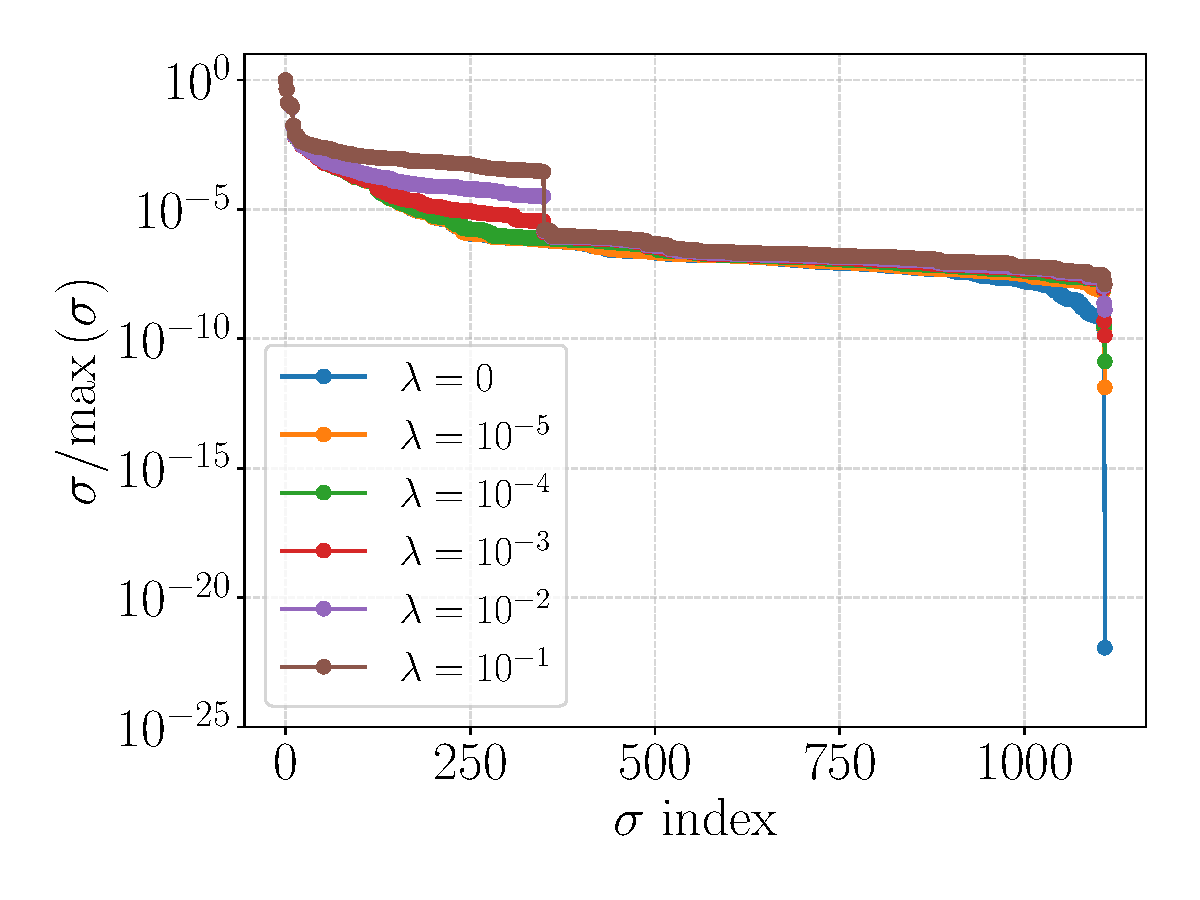
\includegraphics[width=1.0\textwidth]{figures/lm_singular_values_big_new.pdf}
    \caption{Levenberg-Marquardt.}
    \label{subfig:lm}
\end{subfigure}
 \begin{subfigure}[t]{0.49\textwidth}
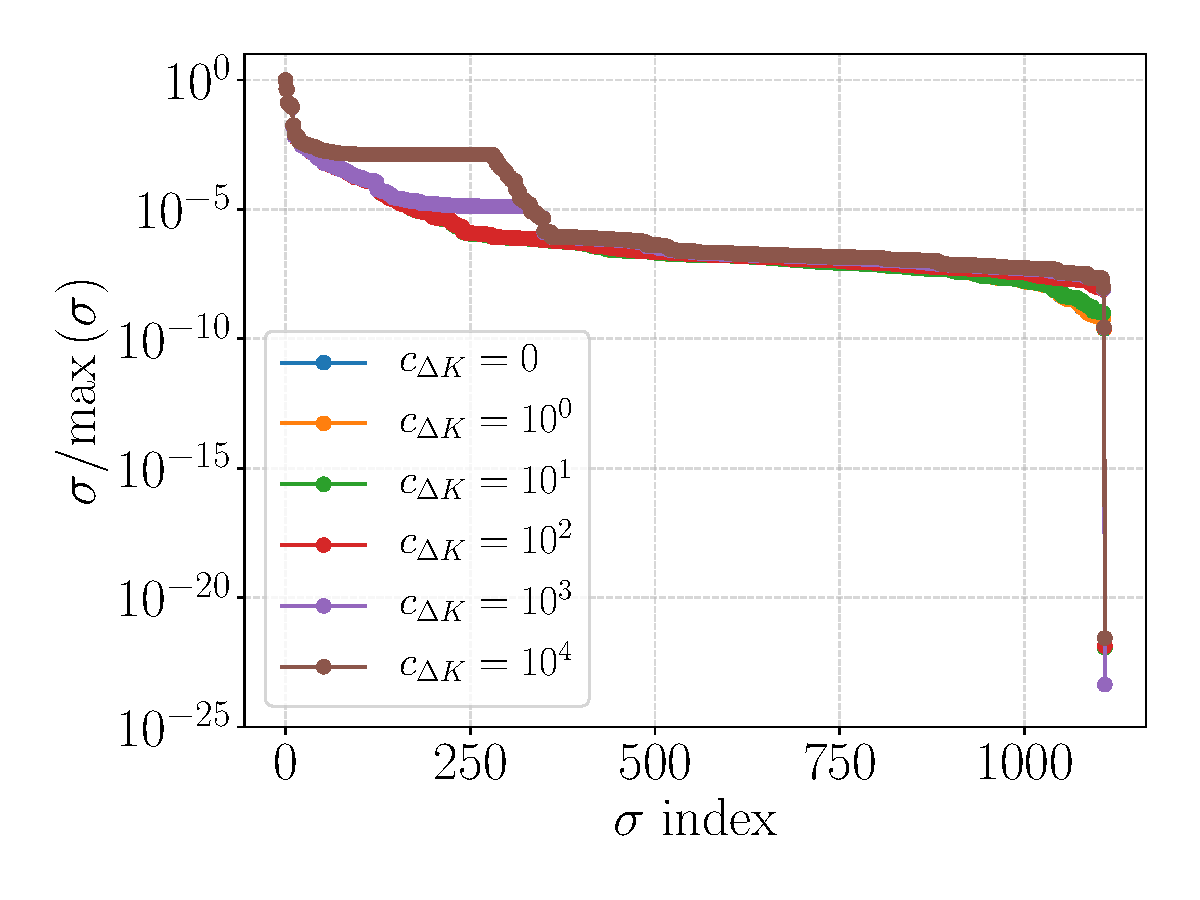
\includegraphics[width=1.0\textwidth]{figures/constraint_singular_values_big_new.pdf}
    \caption{$\Delta K$ constraint, $c_{\Delta K} = w_{\Delta K}/\sigma_{\Delta K}$.}
    \label{subfig:constraint}
\end{subfigure}
\caption{Effect of LM method and $\Delta K$ constraint on singular values of LOCO jacobian matrix.}
\label{fig:singval}
\end{figure}

The jacobian matrix in this analysis includes the~\gls{rf} response elements, i.e., the horizontal dispersion function is included, so the very low singular value $\sim10^{-21}$ for $\lambda = 0$ is related to the degeneracy between the vertical BPMs and correctors gains. With $\lambda = 10^{-5}$ this low singular value is already increased to $\sim10^{-12}$ and the decreasing singular values around $10^{-9}$ in the blue line are also raised. 
% Increasing the value of $\lambda$ introduces a clear step at the $350\ts{th}$ singular value, which is related to the magnet's strengths parameters: $270$ normal quadrupoles plus $80$ skew quadrupoles. The remaining $760$ singular values are related to the BPMs and correctors parameters and their magnitude decreases very slowly. The first $12$ singular values stand out with relative strengths greater than $10^{-2}$ compared to the maximum. These values are related to the $12$ quadrupoles families and since these families are directly related to the lattice periodicity, the first $12$ singular values reflects the importance of the signature of symmetric gradient changes in the~\gls{orm}. 

In the literature~\cite{icfa_huang, huang2013}, it is recommended to start the fitting with $\lambda = 10^{-3}$. From Figure~\ref{subfig:lm} it can be seen that this value raises the singular value at the low end. Increasing $\lambda$ even further raises most of the singular values. Therefore using $\lambda=10^{-3}$ should prevent the problems related to the low singular values while greater values for $\lambda$ produce changes in the singular values that may slow the solution convergence.

Figure~\ref{subfig:constraint} shows the singular values for several constraint magnitudes. The weight vector was set as unity for every element and the normalization constant $\sigma_{\Delta K}$ was changed from $0$ to $10^{-4}$. The case $c_{\Delta K} = 0$ coincide with $\lambda = 0$ in the Figure~\ref{subfig:lm}. The normalization $\sigma_{\Delta K}$ can be interpreted as the limit of step variation in $\Delta K$. The typical values for the quadrupole gradients in Sirius storage ring are on the order of $10^{-2}$. Then setting the constraint on step size to $\Delta K \sim 10^{-2}$ does not really limits the gradients variations and this can be seen in the similar singular values distributions for $c_{\Delta K}$ from $0$ to $10^{2}$. Only with $c_{\Delta K}=10^{3}$ the changes in singular values are substantial. Notice that some singular values at low end are also raised with the $\Delta K$ constraints, these low singular values are related to the quasi-degeneracies between quadrupoles that may lead to large excursions in quadrupole gradients when no constraints are used.

Limiting too much the $\Delta K$ step variation may increase unnecessarily the number of iterations required for LOCO convergence. Hence, in the literature~\cite{icfa_huang, huang2013} it is recommended to use the maximum value of $\sigma_{\Delta K}$ that still produces a significant change in the singular values, aiming to balance the $\Delta K$ constraints and the number of iterations, therefore reducing LOCO running time whenever it is worth it. For Sirius storage ring, the optimum value was determined to be $\sigma_{\Delta K} = 10^{-3}$, thus $c_{\Delta K} = 10^{3}$.

Notice that with $c_{\Delta K}=10^{3}$ the last singular value was relatively smaller compared to the unconstrained case. This can be solved by combining the constrained case with the~\gls{lm} minimization, given that it was seen that the~\gls{lm} contribution raises the singular values. The singular values distribution for the chosen values of $\lambda$ and $c_{\Delta K}$ compared to the original distribution are shown in Figure~\ref{fig:compare_svs}. The last singular value is associated with the gain degeneracy between vertical~\glspl{bpm} and correctors, so, in principle, it is the only singular value that should be removed.
\begin{figure}
\centering
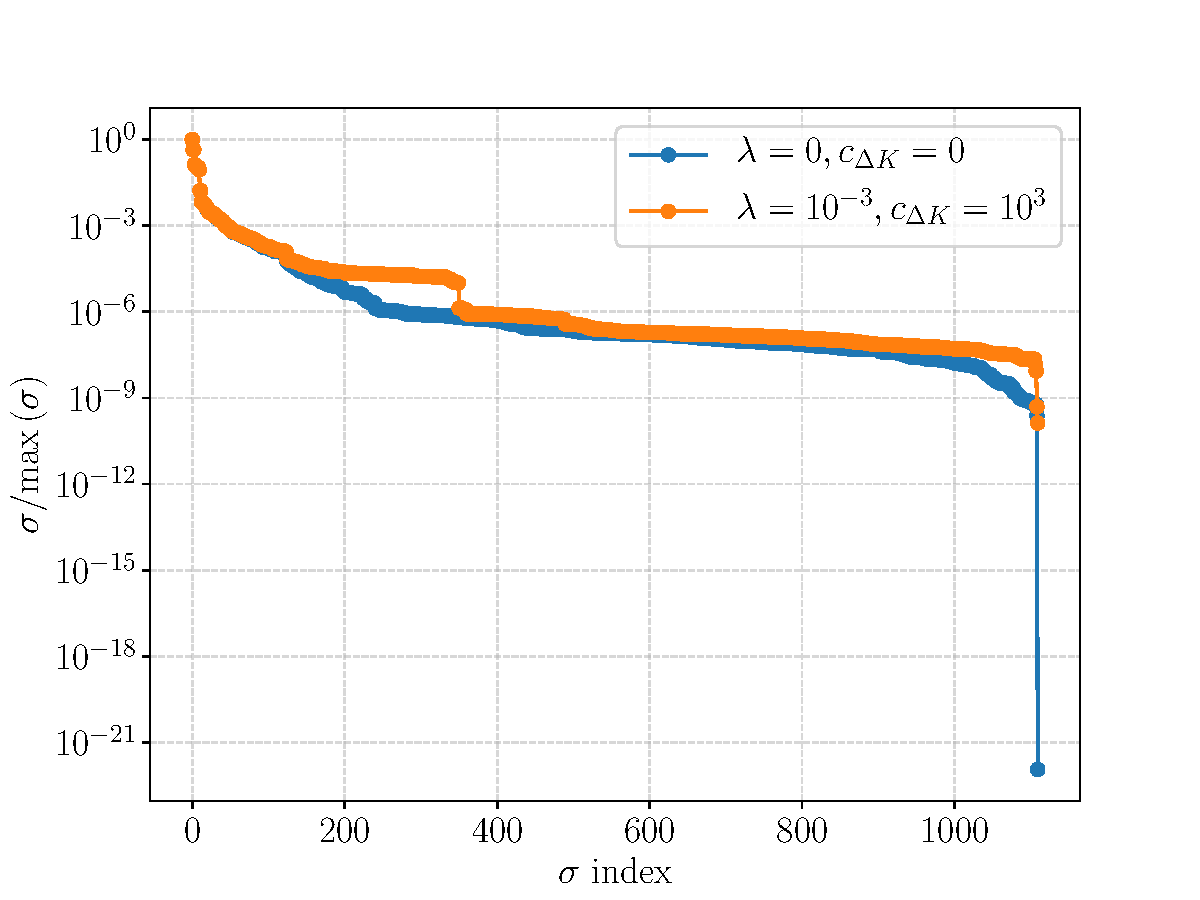
\includegraphics[width=0.70\textwidth]{figures/chosen_singular_values.pdf}
\caption{Singular values distributions between GN unconstrained method and LM constrained method with chosen parameters.}
\label{fig:compare_svs}
\end{figure}
\chapter{Code Implementation for Sirius}
To be written.
% \section{Accelerator Physics codes}
% % \subsection{Matlab Accelerator Toolbox}
% \begin{description}
%     \item[TrackC++:]
%     \item[PyAccel:]
%     \item[PyModels:]
% \end{description}
% \section{Python Implementation}
% \section{Tests}
% \subsection{Perturbations on Simulated Model}
% \subsection{Initial Condition Dependence}
% \subsection{Single Error Detection}







\chapter{Measurements and corrections}

\section{Orbit response matrix}
\section{Transverse Linear Coupling}
\section{Betatron Function}
\section{Dispersion Function}
% \section{Emittance}
\section{Dynamical Aperture}
\section{Injection Efficiency}

% \chapter{Optics measurements}

% Finaliza a parte no bookmark do PDF, para que se inicie o bookmark na raiz
\bookmarksetup{startatroot}%

\chapter*[Conclusions]{Conclusions}
    \addcontentsline{toc}{chapter}{Conclusions}

    In this work, the Linear Optics from Closed Orbit (LOCO) method was studied and implemented as a Python package for the Sirius storage ring. The code was submitted to several tests, using Orbit Response Matrices (ORM) obtained with simulations and measurements performed in the storage ring as well. The tests validated that the implemented method is robust and reliable. In these tests, the use of Levenberg-Marquardt (LM) minimization algorithm instead of Gauss-Newton (GN) proved to be the best choice to facilitate the singular values selection process required for fit parameters calculations. With this choice, only the last singular value, which is related to the well-known gain degeneracy in the vertical plane, should be removed. The LM algorithm has proved to be a great alternative for the time-consuming process of trial and error to determine the best set of singular values to be used in the fitting with GN algorithm. Another very important feature for the method was the constraints in quadrupole's strengths. Without constraints, the fitting converges to unrealistic solutions with large deviations on the gradients in quasi-degenerated quadrupoles (with similar signatures on ORM). Including constraints in step sizes, the solutions obtained reached the same quality of fitting with the advantage of providing much more realistic and feasible gradients variations.
    
    LOCO method was applied in Sirius storage ring to correct the linear optics and coupling. The fit parameters error bars were obtained by measuring and fitting 10 ORMs. An individual quadrupole gradient in the lattice was intentionally changed, the ORM was measured and adjusted to prove that the method was able to accurately recover the localized variation. The ORM measured without optics and coupling corrections on storage ring were adjusted with LOCO with 20 different initial conditions on the quadrupoles gradients and all solutions obtained virtually converged to the same setting of quadrupoles, within the parameters error bars, indicating that the found solution provides the best ORM fit available. With two LOCO iterations, where the corrections were applied in quadrupoles trim-coils and skew quadrupoles at Sirius storage ring, another ORM as measured and adjusted with the method, the measured and nominal ORM difference was reduced from $\chi = \SI{24.6}{\micro\meter}$ to $\SI{2.1}{\micro\meter}$. The errors of on-diagonal ORM blocks were reduced to about \sfrac{1}{9} from its initial values and the off-diagonal blocks related to the coupling were greatly reduced to approximately \sfrac{1}{20} of the initial errors. While the measured BPM accuracy was around $\SI{200}{\nano\meter}$, the LOCO fitting level for the ORM in these iterations was about $\SI{920}{\nano\meter}$. Although a sub-$\SI{}{\micro\meter}$ level of fitting is already satisfactory, this factor of 4 larger than the BPM accuracy indicates that there are still some systematic errors in the storage ring contributing to the ORM measurement that should be investigated. The dispersion functions had to be included in the fitting with a weight factor, otherwise, the differences between measured and fitted horizontal dispersion were very large. The measured vertical dispersion function could not be explained with the calibrated model. 
    
    The final corrections applied in Sirius storage ring for normal gradients covered a range of $\pm\SI{2}{\%}$ and for skew gradients, the range was $\pm\SI{5e-3}{\meter^{-1}}$. Some independent measurements were performed to characterize the storage ring optics, coupling and performance before and after corrections. A summary of the obtained results is presented in Table~\ref{tab:params_corr_summary}.
\begin{table}
    \centering
    \caption{Summary of storage ring parameters before and after LOCO corrections}
    \label{tab:params_corr_summary}
    \begin{tabular}{ccccc}
        \toprule\toprule
        Parameter & Before Corr. & After Corr. & Unit & Improvement Factor\\
        \hline
        $\Delta\beta_x/\beta_x$ (std) & \num{12.8(8)} & \num{3.9(8)} & \SI{}{\%} & \num{3.3} \\
        $\Delta\beta_y/\beta_y$ (std) & \num{10.4(5)} & \num{4.1(5)} & \SI{}{\%} & \num{2.5} \\
        $\Delta\eta_x$ (std) &  \num{10.2(2)} &  \num{1.6(2)} & \SI{}{\milli\meter} & \num{6.4} \\
        $\Delta\eta_y$ (std) &  \num{2.8(3)} &  \num{1.9(3)} & \SI{}{\milli\meter}& \num{1.5} \\
        % Betatron Coupling $|\kappa|$ &  \num{0.78(4)} & \num{0.07(1)} & \SI{}{\%} & \num{11.14} \\
        H. Dynamic Aperture  & \num{7.6} & \num{8.3} & \SI{}{\milli\meter} & \num{1.1} \\
        Injection Efficiency (mean)  & \num{20} & \num{68} & \SI{}{\%} & \num{3.4} \\
        \bottomrule\bottomrule
    \end{tabular}
\end{table}

Regarding the coupling, the measured global betatron coupling was reduced from $\SI{0.78(4)}{\%}$ to $\SI{0.07(1)}{\%}$, proving that LOCO is a robust tool to minimize both the off-diagonal ORM components and the global coupling as well. Initially, the calibrated LOCO model predicted the optics functions quite well compared to the measured values (except for the vertical dispersion). In the last fitting, after corrections application, this correspondence was not observed anymore. 

The orbit contribution to the optics and coupling on Sirius storage ring was also studied. The measured residual orbit with respect to the~\gls{bba} orbit was reproduced in the model. An ORM was calculated in this perturbed model and adjusted with LOCO. The model behavior, in this case, was similar to the obtained in the first iteration in the actual storage ring. The obtained optics errors caused by the orbit distortion in the model via the feed-down effect were on the same order compared to the errors measured in the storage ring without corrections. The horizontal and vertical dispersion function errors in both cases presented a considerable correlation. It was also necessary to include the dispersion function in the fitting with a weight factor to adjust the perturbed model dispersion. The vertical dispersion also could not be explained with LOCO model. The changes in quadrupole gradients and skew quadrupoles to fit the perturbed ORM was also on the order of magnitude of the corrections applied to the machine. All these results indicate that the residual orbit present in Sirius storage ring is perturbing considerably the optics and coupling by feed-down effect on quadrupoles and sextupoles. Moreover, the corrections calculated with LOCO and applied to the machine might be somewhat compensating for these errors generated by the orbit distortion. We concluded that the storage ring status obtained reached the limit allowed for this kind of compensation. To improve even further the parameters, the feed-down effect must be minimized by reducing the residual orbit. At the time of writing, the orbit correction was limited by the correctors kicks thresholds $\pm\SI{330}{\micro\radian}$, which should be sufficient to correct the orbit at the BPMs in a better level, considering the magnet alignment errors tolerances. Measurements in the storage ring indicated that the actual errors were not meeting specifications and a realignment campaign was scheduled for January 2021. After that, it is expected that the residual orbit can be greatly reduced, consequently the related optics perturbations and, applying LOCO method developed in this work, the storage ring linear optics and performance might be further improved towards design values. 
\section*{Future Activities}
The Sirius commissioning is a work in progress and there are many subsequent activities related to this work. As already mentioned, the analysis and corrections of storage ring optics and coupling will be performed after the machine realignment. Once the diagnostic beamline is available, it will be possible to use beam size and emittance measurements as an independent verification for the effect of the corrections on the beam. 

The Python code is planned to be generalized in the way of being able to run with any given lattice model, not only for the Sirius storage ring model. There is also an idea of implementing a graphical user interface in Python for the developed LOCO code, compatible with Sirius control system, then facilitating LOCO configuration setup, fitting, analysis, visualization of results and corrections application on the machine. This would make this LOCO Python version a user-friendly helpful tool for regular operations and machine studies on Sirius. 

LOCO analysis can be performed with ORM measured with different conditions on Sirius storage ring. Different kicks amplitudes can be used in ORM measurements to check the non-linear contributions to the matrix. The effects of measuring ORMs different energy deviations (off-energy orbits) may also be studied. The sextupoles setup can be varied to change the betatron tunes dependence with energy deviations (the chromaticity) in the ORM measurements and LOCO fittings.

Since the ORM measurement process takes about 40 minutes, the obtained data is subjected to drifts in the machine which may add errors to the ORM. Other facilities implemented a much faster and accurate ORM measurement, exciting the beam orbit with different known frequencies oscillations on correctors kicks. Applying Fourier analysis on the data, the ORM elements can be obtained. With this method the ORM can be measured in a few minutes and LOCO analysis can be applied, then reducing the overall time required for Sirius optics studies.

ORM can be measured with different currents per bunch in the electron beam. The corresponding LOCO fitting for each measurement can provide information about the transverse impedance distribution around Sirius storage ring.  
Another branch of study is to benchmark LOCO results and corrections with other methods, for example, methods based on~\gls{tbt} data acquired from~\glspl{bpm}, such as~\gls{pca} and Independent Component Analysis (ICA), which also fits optics function in the lattice model and provides variations in fit parameters that can be applied as corrections on the machine.
% --------- Elementos pós-textuais --------------&
\postextual

\appendix

\chapter{Singular Value Decomposition - SVD}\label{appendix:svd}

Let $\mathbf{M}$ be a real $m \times n$ matrix. The Singular Value Decomposition (SVD) is a factorization that generalizes the eigenvalues decomposition and it states that every matrix can be decomposed in the following form:

\begin{equation}
    \mathbf{M} = \mathbf{U} \Sigma \mathbf{V}^{\mathsf{T}},
    \label{eq:svd}
\end{equation}

where $\mathbf{U}$ is a $m \times m$ matrix, $\mathbf{V}$ is a $n \times n$ matrix and $\Sigma$ is a $m \times n$ positive-definite rectangular diagonal matrix. $\mathbf{U}$ and $\mathbf{V}$ are orthogonal matrices:

\begin{align}
    \mathbf{U}\mathbf{U}^{\mathsf{T}} = \mathbf{U}^{\mathsf{T}}\mathbf{U} &= \mathbf{I}_{m} \\
    \mathbf{V}\mathbf{V}^{\mathsf{T}} = \mathbf{V}^{\mathsf{T}}\mathbf{V} &= \mathbf{I}_{n}. 
\end{align}

Manipulating the equation \eqref{eq:svd} and using the matrices properties we obtain

\begin{align}
    \mathbf{M}\mathbf{M}^{\mathsf{T}} &= \mathbf{U} \Sigma^2 \mathbf{U}^{\mathsf{T}} \\
    \mathbf{M}^{\mathsf{T}}\mathbf{M} &=  \mathbf{V} \Sigma^2 \mathbf{V}^{\mathsf{T}}.
\end{align}

From this, we observe that the diagonal elements of $\Sigma^2$ are eigenvalues of $\mathbf{M}\mathbf{M}^{\mathsf{T}}$ and $\mathbf{M}\mathbf{M}^{\mathsf{T}}$, which are called row-wise correlation and column-wise correlation matrices, respectively. Since $\mathbf{U}^{\mathsf{T}} = \mathbf{U}^{-1}$ and $\mathbf{V}^{\mathsf{T}} = \mathbf{V}^{-1}$, the columns of $\mathbf{U}$ are the eigenvectors of $\mathbf{M}\mathbf{M}^{\mathsf{T}}$ and the columns of $\mathbf{V}$ are the eigenvectors of $\mathbf{M}^{\mathsf{T}}\mathbf{M}$.

The diagonal elements $\sigma_i := \Sigma_{ii} \geq 0$ are called singular values. The SVD of a matrix is not unique but a default choice is to arrange the decomposition in such a way that the singular values are sorted in descending order, $\sigma_i \geq \sigma_j$ for $i < j$. The number of non-zero singular values is exactly the rank of matrix $\mathbf{M}$. Thus, the SVD of a rank deficient matrix will result in zero or numerically very small singular values. 

A common procedure to avoid degeneracies in the calculations is the singular values selection. This can be done by setting explicitly the unwanted singular values to zero. This can be done in a more insightful way by defining a minimum threshold $\delta$ and setting to zero the singular values that satisfy $\dfrac{\sigma_i}{\mathrm{max}\left(\sigma_i\right)} < \delta$. This methods eliminates the less important directions defined by the columns of $\mathbf{U}$ and $\mathbf{V}$ as compared to the direction with higher singular values. 

Since $\Sigma$ is a square diagonal matrix, its inverse is obtained simply by $\Sigma^{-1}_{ii} = 1/\sigma_{i}$. For the case that $\sigma_{i} = 0$, one can define $\Sigma^{-1}_{ii} = 0$. Hence, the matrix $n \times m$

\begin{equation}
    \mathbf{M}^{-1} = \mathbf{V} \Sigma^{-1} \mathbf{U}^{\mathsf{T}},
    \label{eq:svd_inverse}
\end{equation}

is the pseudo-inverse of $\mathbf{M}$ as can be checked by

\begin{align}
    \mathbf{M}^{-1}\mathbf{M} =  \left(\mathbf{V} \Sigma^{-1} \mathbf{U}^{\mathsf{T}} \right)\left(\mathbf{U} \Sigma \mathbf{V}^{\mathsf{T}}\right) &= \mathbf{I}_{n} \\
    \mathbf{M}\mathbf{M}^{-1} =  \left(\mathbf{U} \Sigma \mathbf{V}^{\mathsf{T}}\right)\left( \mathbf{V} \Sigma^{-1} \mathbf{U}^{\mathsf{T}} \right)&= \mathbf{I}_{m}. 
\end{align}

The matrix $\mathbf{M}^{-1}$ is also known as Moore-Penrose pseudo-inverse \cite{numerical_recipes}.

A useful version of SVD is the so-called ``economy SVD''. Let $r = \mathrm{min}\left(m, n\right)$, then one can observe that $\sigma_i = 0$ for $i > r$. In this way, all these diagonal zeros in the rectangular $m \times n$ matrix $\Sigma$ can be removed to build a smaller square matrix $\hat{\Sigma}$ with dimension $r \times r$. Doing that allows for reducing the dimension of $\mathbf{U}$ as well, obtaining a rectangular $m \times r$ matrix $\hat{\mathbf{U}}$. The matrix $\mathbf{V}$ is unchanged. In this version, the new matrix $\hat{\mathbf{U}}$ is semi-orthogonal, i.e., $\hat{\mathbf{U}}^{\mathsf{T}}\hat{\mathbf{U}} = \mathbf{I}_r$ but $\hat{\mathbf{U}}\hat{\mathbf{U}}^{\mathsf{T}} \neq \mathbf{I}_m$ in general. The economy SVD is very interesting for numerical purposes, since it is common that $m \gg n$ or $m \ll n$, then using only the minimum useful data contained in the SVD matrices is very computationally beneficial.

The \gls{svd} pseudo-inversion is a powerful tool to solve generic linear systems of equations given by

\begin{equation}
    \mathbf{A} \vec{x} = \vec{b},
    \label{eq:linear_system}
\end{equation}

where $\mathbf{A}$ is a $m \times n$ matrix, $\vec{x}$ a $n \times 1$ column vector and $\vec{b}$ a $m \times 1$ column vector. The case that $m=n$ may be exactly solvable, if $\mathrm{det}\left(\mathbf{A}\right) \neq 0$ the exact solution is obtained by normal inversion. Other two cases that may not have an exact solution occur:

\begin{itemize}
    \item Underdeterminated: $m < n$ and the system has infinitely many solutions, given a generic vector $\vec{b}$. The system does not have enough information given by the elements of $\vec{b}$ to obtain the exact unknowns $\vec{x}$. With the pseudo-inversion it is possible to obtain a solution $\vec{x}_s$ to the linear system such that $|\vec{x}_s|^2 = \sum_{i=1}^{n}x^2_{s, i}$ is minimized. This is called the minimum-norm solution.
    
    \item Overdeterminated: $m > n$ and the system has no solution, given a generic vector $\vec{b}$. The system has more equations than unknowns, so the system is overconstrained and it is not possible to satisfy exactly and simultaneously all the equations. In this case, with the pseudo-inversion it is obtained an approximate solution $\vec{x}_s$ that minimizes the difference $|\mathbf{A}\vec{x}_s - \vec{b}|$. This is called the least squares solution.
\end{itemize}









\chapter{BPMs and correctors gains matrices}\label{appendix:gains}

% Referências bibliográficas
% \bibliographystyle{unsrt}
% \bibliographystyle{numeric}
% \bibliographystyle{plain}
\bibliography{library}
% \printbibliography


% % Apêndices
% \begin{apendicesenv}
% % Imprime uma página indicando o início dos apêndices
% \partapendices
%
% \chapter{Catch up Distance}\label{app:catch_up}
\end{document}